\documentclass[10pt,a4paper]{article}
\usepackage[OT1]{fontenc}
\usepackage[cp1252, utf8]{inputenc}
\usepackage{amsmath}
\usepackage{amsfonts}
\usepackage{amssymb}
\usepackage{xcolor}
\usepackage{graphicx}
\usepackage{braket}
\usepackage{bm}
\usepackage{listings}
\usepackage[most]{tcolorbox}
\usepackage{fancyvrb}
\usepackage{standalone}

\definecolor{keywordpurple}{RGB}{100,65,150}
\definecolor{commentgreen}{RGB}{35,170,40}
\lstset{language=[90]Fortran,
  basicstyle=\ttfamily,
  columns=fullflexible,
  keepspaces=true,
  keywordstyle=\color{keywordpurple},
  commentstyle=\color{commentgreen}
}
\usepackage[%
  colorlinks=true,
  urlcolor=blue,
  linkcolor=blue,
  citecolor=blue
]{hyperref}
\usepackage{geometry}
\geometry{
  a4paper,
  total= {170mm,257mm},
  left = 2cm,
  top  = 2cm,
}

\tcbset{colback=blue!10!white}
\tcbsetforeverylayer{colframe=blue!75!black}

\newtcolorbox{codebox}[1]{
  colback=white!5!white,
  colframe=white!75!black,
  title=#1,
  box align=top,
  enhanced,
  breakable,
}

\hbadness=10000

\title{SsTC library:\\
\large{User Guide}\\
\large{Version 0.4.0}}
\author{Álvaro R. Puente-Uriona}
\date{\today}

\graphicspath{{./images}}

%Set font size for figures.
%This is a global parameter to change the label size on all the figures.
\newcommand\imglabelsize{10} %Default: 10.
%

%\usepackage{draftwatermark}
%\SetWatermarkText{DRAFT}
%\SetWatermarkScale{5}

\begin{document}
\maketitle
\tableofcontents
\clearpage
\newpage
\section{Scope}
Solid-state Task Constructor (SsTC) is a high-performance computing (HPC) oriented Fortran 2018 library which aims to aid programmers and researchers in the process of sampling and integration of functions in the first Brillouin zone (BZ) of a given crystalline system. The library is centred around the following concepts:
\begin{tcolorbox}\begin{itemize}
\item The calculator: A general function representing a physical quantity of interest to the user. It is of the form
\begin{equation}\label{eq:calculator}
C^{\bm{\alpha}}(\bm{k}; \bm{\beta}),
\end{equation}
where $\bm{k}$ is a vector in the BZ and $\bm{\alpha}, \bm{\beta}$ encompass \textit{all} other functional dependences of $C$. In the document we refer to $\bm{\alpha}$ as integer or discrete indices and seek to represent, for example, a set of Cartesian components $\{x, y, z\}$ or band indices. On the other side, $\bm{\beta}$ are referred as continuous indices and seek to represent the dependence of $C$ on non-intrinsic variables such as an externally controlled frequency $\omega$ or a variable range of Fermi energies $\varepsilon_F$.
\item The task: An object containing a complete description of the calculator $C$ and the sampling or integration task that the programmer wants to perform.
\item The system: An object containing a complete description of a crystalline system given by its tight-binding \cite{marzariMaximallyLocalizedWannier2012} representation. This includes:
\begin{tcolorbox}\begin{itemize}
\item Number of bands.
\item Fermi energy.
\item Unit cell description: the projection of lattice vectors $\bm{a}_i$ in the $\{x, y, z\}$ axes in units of \r{A}.
\item Resolution of the Hamiltonian operator $\hat{H}$ in the basis of the Wannier functions (WFs) \cite{marzariMaximallyLocalizedWannier2012} in units of eV, i.e., the on-site and tunnelling amplitudes.
\item Resolution of the position operator $\hat{\bm{r}}$ in the basis of the WFs in units of \r{A}.
\end{itemize}\end{tcolorbox}
\end{itemize}
\end{tcolorbox}
The sampling and integration utilities contained in SsTC are the following.
\begin{tcolorbox}\begin{itemize}
\item ``Kpath" sampling. 1-dimensional sampling of $C$ with specification of the path to sample.
\item ``Kslice" sampling. 2-dimensional regular sampling of $C$ with specification of the slice to sample.
\item ``Regular" sampling. 3-dimensional regular sampling of $C$ with specification of the number of samples in each dimension.
\item Integration. 3-dimensional regular sampling of $C$ followed by an integration process. The integration process as for v0.4.0 amounts to the rectangle approximation or extrapolation methods in each dimension.
\end{itemize}\end{tcolorbox}
All the concepts covered in this section are treated with greater detail in the specific sections in the document.
\section{Prerequisites, installation \& linking to application}\label{sec:install}
SsTC is a Fortran 2018 standard complying code and the prerequisites for its compilation are,
\begin{tcolorbox}\begin{itemize}
\item Any implementation of BLAS, LAPACK, OpenMP and MPI libraries. We recommend those provided by the Intel oneAPI toolkit (Math Kernel Libraries (MKL), OpenMP and MPI).
\item Intel Fortran oneAPI compilers \verb|ifort| or \verb|ifx| or GNU Fortran compiler \verb|gfortran|.
\item Python 3 software with 're' and 'glob' libraries.
\end{itemize}\end{tcolorbox}
As for v0.4.0, SsTC is only guaranteed to compile on Linux systems using the above mentioned compilers contained in the \href{https://www.intel.com/content/www/us/en/developer/tools/oneapi/hpc-toolkit.html}{Intel\textregistered oneAPI HPC} toolkit and the \verb|gfortran| compiler. As such, the main application to be linked with must be compiled with the MPI wrappers \verb|mpiifort|, \verb|mpiifx| or \verb|mpif90|.

The SsTC project is hosted on \href{https://github.com/irukoa/SsTC}{GitHub} and can be downloaded by running the command,

\begin{codebox}{Download}
\begin{verbatim}
git clone --recurse-submodules https://github.com/irukoa/SsTC.git
\end{verbatim}
\end{codebox}
or by downloading a compressed version of the source code on the \href{https://github.com/irukoa/SsTC/tags}{tag history}.

To install the source code, move the \verb|SsTC| folder to a path of your choice and run \verb|make|.
\begin{codebox}{Installation}
\begin{verbatim}
bash:/current/dir$ mv SsTC/ /path/of/your/choice/
bash:/path/of/your/choice$ cd SsTC/
bash:/path/of/your/choice/SsTC$ make
\end{verbatim}
\end{codebox}
These commands will compile the source code and install the library \verb|libSsTC.a| and the module header file \verb|sstc.mod| in the directory \verb|/path/of/your/choice/SsTC/bin/|.

The default behaviour will compile the library with \verb|mpiifort|, but the user can also employ \verb|mpiifx|/\verb|mpif90| to compile. This can be achieved by running,
\begin{codebox}{Installation using ifx}
\begin{verbatim}
bash:/path/of/your/choice/SsTC$ cp config/ifx Makefile
bash:/path/of/your/choice/SsTC$ make
\end{verbatim}
\end{codebox}
or
\begin{codebox}{Installation using gfortran}
\begin{verbatim}
bash:/path/of/your/choice/SsTC$ cp config/gfortran Makefile
bash:/path/of/your/choice/SsTC$ make
\end{verbatim}
\end{codebox}
which will replace the Makefile for compilation with \verb|mpiifort| by the one for compilation with \verb|mpiifx|/\\ \verb|mpif90| and build the library.

To link to your Fortran application \verb|appl.F90|, add the line \verb|use SsTC| in your application preamble and compile with
\begin{codebox}{Compilation \& Linking}
\begin{verbatim}
bash:/path/to/application/$ $(F90) $(F90FLAGS) appl.F90
-I/path/of/your/choice/SsTC/bin
/path/of/your/choice/SsTC/bin/libSsTC.a -o "appl.x"
\end{verbatim}
\end{codebox}
where \verb|F90 = mpiifort/mpiifx/mpif90| and \verb|F90FLAGS| contains, at least,
\begin{codebox}{Compilation flags}
\begin{verbatim}
F90FLAGS = -qopenmp -lmkl_intel_lp64 -lmkl_core -lmkl_gnu_thread -pthread
\end{verbatim}
\end{codebox}
or the compiler specific analogues of the above mentioned flags.

To make use of SsTC, the application preamble of \verb|appl.F90| should also contain the lines
\begin{codebox}{Use statements}
\begin{verbatim}
use MPI_F08
use OMP_LIB
\end{verbatim}
\end{codebox}
The application must also contain a call to the MPI \cite{messagepassinginterfaceforumMPIMessagePassingInterface2021} initialization routine \verb|call MPI_INIT(ierror)| followed by a call to the SsTC initialization routine \verb|call SsTC_init()| \textit{before} any call to other SsTC routines. The programmer also needs to make sure that the MPI finalizing routine \verb|call MPI_FINALIZE(ierror)| has not been called before using SsTC routines.

Note:  By default, SsTC uses double precision numbers for real and complex valued scalars and arrays.

The application \verb|appl.x| can be run by the commands
\begin{codebox}{Running}
\begin{verbatim}
/path/to/application/appl.x
mpirun -np $N /path/to/application/appl.x
\end{verbatim}
\end{codebox}

To uninstall the library run
\begin{codebox}{Uninstalling}
\begin{verbatim}
 bash:/path/of/your/choice/SsTC$ make uninstall
\end{verbatim}
\end{codebox}
\section{Calculators \& tasks}
The calculator Eq. \eqref{eq:calculator} is the generic name for Fortran function with interface
\begin{codebox}{}
\begin{lstlisting}[caption={Interface of a global calculator.},captionpos=b, label={lst:interface_g_calc}]
abstract interface
  function SsTC_global_calculator(task, system, k, error) &
           result(u)
    class(SsTC_global_k_data), intent(in) :: task
    type(SsTC_sys), intent(in)            :: system
    real(kind=dp), intent(in)             :: k(3)
    !In coords. relative to recip. lattice vectors.
    logical, intent(inout)                :: error

    complex(kind=dp) :: u(product(task%integer_indices), &
                          product(task%continuous_indices))
  end function SsTC_global_calculator
end interface
\end{lstlisting}
\end{codebox}
given by external SsTC modules, see Sec. \ref{sec:modularity}, or otherwise provided by the user in the scope of the main application using SsTC. The calculator must be interface conforming.

Additionally to the general ``global calculator", there exists a ``local calculator" with interface
\begin{codebox}{}
\begin{lstlisting}[caption={Interface of a local calculator.},captionpos=b, , label={lst:interface_l_calc}]
abstract interface
  function SsTC_local_calculator(k_data, system, k, error) &
           result(u)
    class(SsTC_local_k_data), intent(in) :: k_data
    type(SsTC_sys), intent(in)           :: system
    real(kind=dp), intent(in)            :: k(3)
    !In coords. relative to recip. lattice vectors.
    logical, intent(inout)               :: error

    complex(kind=dp) :: u(product(k_data%integer_indices))
  end function SsTC_local_calculator
end interface
\end{lstlisting}
\end{codebox}
with reduced functionality and meant for internal computations regarding quantities local for each $\bm{k}$ point, as described in Sec. \ref{sec:local_k_quantities}.

The task is a Fortran object (derived type) of \verb|class(SsTC_local_k_data)|, of which \\ \verb|type(SsTC_global_k_data)| is an extension, specifying the sampling or integration task to perform and contains a full description of the properties of the calculator $\bm{\alpha},\bm{\beta}$. The generic properties which apply to every task \verb|task| are the following,
\begin{tcolorbox}[enhanced, breakable]\begin{itemize}
\item \verb|character(len=*) :: task%name|: The name given to the task.
\item \verb|procedure(SsTC_global_calculator), pointer :: task%global_calculator|: Interface conforming procedure pointer to the selected calculator. The library's sampling routines will use the provided calculator to sample.
\item \verb|procedure(SsTC_local_calculator), pointer :: task%local_calculator|: Interface conforming procedure pointer to the selected calculator. The library's sampling routines will use the provided calculator to sample. Note: only one of \verb|task%local_calculator| or \verb|task%global_calculator| shall be associated when sampling.
\item \verb|integer :: task%integer_indices(N_int_ind)|: Each entry \verb|i| of the array contains the number of values the integer index $\alpha_i$ in Eq. \eqref{eq:calculator} can have. \verb|N_int_ind| is the total number of integer indices encompassed by $\bm{\alpha}$ and the total number of integer index combinations is given by \verb|product(task%integer_indices)|.
\item \verb|integer :: task%continuous_indices(N_ext_vars)|: Each entry \verb|i| of the array contains the number \verb|ext_vars_steps(i)| of values the continuous index $\beta_i$ in Eq. \eqref{eq:calculator} can have. \verb|N_ext_vars| is the total number of external variables encompassed by $\bm{\beta}$ and the total number of continuous index combinations is given by \verb|product(task%continuous_indices)|. Not applicable to \verb|type(SsTC_local_k_data)|.
\item \verb|real(kind=dp) :: task%ext_var_data(N_ext_vars)%data(ext_vars_steps(N_ext_vars))|: Each entry \verb|i, j| corresponding to \verb|task%ext_var_data(i)%data(j)| is a real number $\lambda_{ij}$ containing the particular value the continuous index $\beta_{i}$ has, as given by
\begin{equation}\label{eq:disc_cont}
\lambda_{ij} = \lambda_{i1} + \left(\lambda_{i\;\verb|ext_vars_steps(i)|} - \lambda_{i1}\right)\times\left(j - 1\right)/\left(\verb|ext_vars_steps(i)| - 1\right).
\end{equation}
where $\lambda_{i1}$ and $\lambda_{i\;\verb|ext_vars_steps(i)|}$ are the starting and ending points of the values given to $\beta_{i}$, $j\in [1, \verb|ext_vars_steps(i)|]$. Not applicable to \verb|type(SsTC_local_k_data)|.
\end{itemize}\end{tcolorbox}
Particular tasks can be created by means of a specific sampling or integrator task constructor as described in Sec. \ref{sec: sampling_integration} or by the programmer with complete freedom. Extension of the task members is also possible by means of derived type extension.

In the following we provide the type declarations of \verb|SsTC_local_k_data| and \verb|SsTC_global_k_data|,
\begin{codebox}{Global k data}
\begin{lstlisting}[caption={Derived type corresponding to ``local k data".},captionpos=b]
type SsTC_local_k_data
  character(len=120)                                :: name
  integer, allocatable                              :: integer_indices(:)
  !Each entry contains the range of each of the integer indices.
  complex(kind=dp), allocatable                     :: k_data(:)
  !Data local for each k with integer index in memory array.
  procedure(SsTC_local_calculator), pointer, nopass :: local_calculator => null()
  !Pointer to the local calculator.
  integer                                           :: particular_integer_component &
                                                       = 0
  !Specification of some integer component.
end type SsTC_local_k_data
\end{lstlisting}
\end{codebox}
\begin{codebox}{Local k data}
\begin{lstlisting}[caption={Derived type corresponding to ``global k data".},captionpos=b]
type, extends(SsTC_local_k_data) :: SsTC_global_k_data
  integer, allocatable                               :: continuous_indices(:)
  !Each entry contains the range of each continuous indices.
  type(SsTC_external_vars), allocatable              :: ext_var_data(:)
  !External variable data.
  procedure(SsTC_global_calculator), pointer, nopass :: global_calculator => null()
  !Pointer to the global calculator.
  integer, allocatable                               :: iterables(:, :)
  !Iterable dictionary.
end type SsTC_global_k_data
\end{lstlisting}
\end{codebox}
\section{SsTC initialization}
SsTC can be initialized in the application by using the routine \verb|SsTC_init()|.
\begin{codebox}{SsTC initializer}
\begin{lstlisting}[caption={Interface of ``SsTC initialization".},captionpos=b]
subroutine SsTC_init(nThreads, exec_label)

  integer, intent(in), optional :: nThreads
  !Default are max available threads per MPI process.
  logical, intent(in), optional :: verb !Default .true.
  character(len=*), intent(in), optional :: exec_label !Default "SsTC_exec".

end subroutine SsTC_init
\end{lstlisting}
\end{codebox}
The routine will check whether the MPI library has been initialized and stop the program on execution if it was not. It will also open the output and error log files \verb|file=trim(exec_label//".out")| and \\ \verb|file=trim(exec_label//".err")|. This feature, however, can be disabled by using \verb|verb = .false.| which is useful if SsTC is to be used \textit{within} a parallel environment. Lastly, \verb|nThreads| sets the number of threads per MPI process, with the default value of \verb|OMP_GET_MAX_THREADS()|.
\section{Notation: Memory layout and array layout}\label{sec:notation}
These concepts apply to $N$-dimensional jagged arrays such as \verb|array(:, :, ..., :)|, where each dimension $i$ has size $s_i$. The total size of \verb|array| is
\begin{equation}
\verb|size(array)| = \prod_{i=1}^N s_i.
\end{equation}
An array with such a shape is said to be in ``array layout". In tandem this layout, we consider now the 1-dimensional array \verb|mem(:)|, with the same size as \verb|array|. The array \verb|mem(:)| is defined as the ``memory layout" counterpart of the array \verb|array| if
\begin{equation}
\verb|mem(r)| = \verb|array(n_1, n_2, ..., n_N)|,
\end{equation}
with
\begin{equation}\label{eq:column_mayor_mapping}
r = n_1 + s_1\left(n_2 + s_2\left(n_3 + \cdots\right)\cdots\right) = \sum_{i=1}^N n_i\times \left(\prod_{j=1}^{i-1}s_j\right).
\end{equation}
This mapping is called the \href{https://eli.thegreenplace.net/2015/memory-layout-of-multi-dimensional-arrays}{column mayor} array to memory index mapping. It provides an invertible relation
\begin{equation}
r \Leftrightarrow \{n_1, n_2, \cdots, n_N\},
\end{equation}
which makes it possible to keep track of the elements of an array in both layouts, provided that the sizes of each dimension, $s_i$, are known. The output values of the calculator interfaces, corresponding to the sampling $C^{\bm{\alpha}}(\bm{k}; \bm{\beta})$ for a $\bm{k}$ vector, are always arrays in memory layout, both for integer and continuous indices, which makes the interface of the calculator flexible for any number of integer or continuous indices.

In SsTC, the sizes $s_i$ of integer or continuous indices are specified by the components of \\ \verb|task%integer_indices| and \verb|task%continuous_indices| (if applicable) of the task \\ \verb|class(SsTC_local_k_data) :: task|, respectively. The library provides the jagged array indexing utilities
\begin{tcolorbox}[enhanced, breakable]
\begin{itemize}
\item \verb|SsTC_integer_array_element_to_memory_element|: Returns $r = f(\{n_1, n_2, \cdots, n_N\})$ for integer indices.
\item \verb|SsTC_integer_memory_element_to_array_element|: Returns $\{n_1, n_2, \cdots, n_N\} = f^{-1}(r)$ for integer indices.
\item \verb|SsTC_continuous_array_element_to_memory_element|: Returns $r = f(\{n_1, n_2, \cdots, n_N\})$ for continuous indices.
\item \verb|SsTC_continuous_memory_element_to_array_element|: Returns $\{n_1, n_2, \cdots, n_N\} = f^{-1}(r)$ for continuous indices.
\end{itemize}
\end{tcolorbox}
where $f$ is a function representing the mapping Eq. \eqref{eq:column_mayor_mapping} and $f^{-1}$ represents its inverse mapping. The four utilities are described in detail in Sec. \ref{sec:data_structures}.
\section{Systems}
A system is a Fortran derived type
\begin{codebox}{Crystalline systems}
\begin{lstlisting}[caption={Derived type corresponding to a system.},captionpos=b]
type SsTC_sys
  character(len=120)            :: name
  integer                       :: num_bands
  real(kind=dp)                 :: direct_lattice_basis(3, 3)               
  !Direct lattice basis vectors in A.
  !1st index is vector label, 2nd index is vector component.
  real(kind=dp)                 :: reciprocal_lattice_basis(3, 3)           
  !Reciprocal lattice basis vectors in A^-1.
  !1st index is vector label, 2nd index is vector component.
  real(kind=dp)                 :: metric_tensor(3, 3)
  !Metric tensor of the direct lattice basis.
  real(kind=dp)                 :: cell_volume
  integer                       :: num_R_points
  !Number of R points (unit cells).
  integer, allocatable          :: R_point(:, :)
  !Id of the R-point (1st index) and R-vector coords.
  !relative to the direct lattice basis vectors (2nd index).
  integer, allocatable          :: deg_R_point(:)
  !Degeneracy of the R-point specified by its memory layout id.
  complex(kind=dp), allocatable :: real_space_hamiltonian_elements(:, :, :)
  !Hamiltonian matrix elements (1st and 2nd indexes) and
  !id of the R-point (3rd index) in eV.
  complex(kind=dp), allocatable :: real_space_position_elements(:, :, :, :)
  !Position operator matrix elements (1st and 2nd indexes),
  !Cartesian coordinate (3rd index) and id of the R-point (4th index) in A.
  real(kind=dp)                 :: e_fermi = 0.0_dp
  !Fermi energy.
  real(kind=dp)                 :: deg_thr = 1.0E-4_dp
  !Degeneracy threshold in eV.
  real(kind=dp)                 :: deg_offset = 0.04_dp
  !Offset for regularization in case of degeneracies, in eV.
end type SsTC_sys
\end{lstlisting}
\end{codebox}
representing a crystalline system by its tight-binding \cite{marzariMaximallyLocalizedWannier2012} representation. The components
\begin{equation}
\verb|real_space_hamiltonian_elements(m, n, id)| = \braket{m\bm{0}|\hat{H}|n\bm{R}},\quad \verb|id|\;\text{corresponds to }\bm{R}.
\end{equation}
and
\begin{equation}
\verb|real_space_position_elements(m, n, i, id)| = \braket{m\bm{0}|\hat{r}_i|n\bm{R}},\quad \verb|id|\;\text{corresponds to }\bm{R}.
\end{equation}
are identified.
The recommended way to create system is by using the function \verb|SsTC_sys_constructor|,
\begin{codebox}{System constructor}
\begin{lstlisting}[caption={Interface of the system constructor.},captionpos=b]
function SsTC_sys_constructor(name, path_to_tb_file, &
                              efermi, deg_thr, deg_offset) &
  result(system)

  character(len=*), intent(in)        :: name
  character(len=*), intent(in)        :: path_to_tb_file
  real(kind=dp), optional, intent(in) :: efermi, &
                                         deg_thr, deg_offset

  type(SsTC_sys) :: system
end function SsTC_sys_constructor
\end{lstlisting}
\end{codebox}
where the optional arguments can be specified. The function will try to read a file named \\ \verb|trim(path_to_tb_file)//trim(name)//"_tb.dat"| in the path relative to the main application directory. The files have the format of a \href{https://wannier.org/}{Wannier90} \cite{pizziWannier90CommunityCode2020} \href{https://raw.githubusercontent.com/wannier-developers/wannier90/v3.1.0/doc/compiled_docs/user_guide.pdf}{tight-binding} (\verb|*_tb.dat| file, see Sec. 8.21 of the Wannier90 user's guide for v3.1.0) which can be written by the user for toy tight-binding models or can be generated by the code Wannier90 from postprocessing \textit{ab-initio} calculations. As for v3.1.0 of Wannier90, the file is automatically generated when running \verb|wannier90.x| if the option \verb|write_tb=.TRUE.| is specified in the Wannier90 input card (\verb|*.win| file).
\section{Sampling and integration routines}\label{sec: sampling_integration}
In this section we describe the main routines of the SsTC library, encompassing task creation, task sampling or integration and printing to files. Note that the sampling or integration subroutines take as inputs tasks corresponding to the same \verb|class| as the tasks generated by the respective task constructors, which are, at the same time, extensions of \verb|type(SsTC_global_k_data)|. As such, much flexibility in the definition of calculators can be achieved by means of type extension.
\subsection{Kpath module}
This module is centered around creating, sampling, and printing tasks which involve a path in reciprocal space. The ``kpath" task is a derived type
\begin{codebox}{Kpath task}
\begin{lstlisting}[caption={Derived type corresponding to a ``kpath" task.},captionpos=b]
type, extends(SsTC_global_k_data) :: SsTC_kpath_task
  !1st index is the id of the vector in the path.
  !2nd index corresponds to the component of the vector
  !in the path in coordinates relative to the reciprocal lattice.
  real(kind=dp), allocatable :: vectors(:, :)
  !number_of_pts(i) contains the number of k-points between vector i and vector i+1.
  integer, allocatable :: number_of_pts(:)
  !Array to store data with integer index,
  !continuous index and kpt index respectively.
  complex(kind=dp), allocatable :: kpath_data(:, :, :)
end type SsTC_kpath_task
\end{lstlisting}
\end{codebox}
where we consider a set of $N$ reciprocal space vectors $\{\bm{q}_i, i\in[1, N]\}$ by their components $\{a_{ij}\}$ relative to the reciprocal space basis vectors $\bm{b}_{\{1, 2, 3\}}$,
\begin{equation}\label{eq:vec_coords_path}
\bm{q}_i = \sum_{j=1}^3 a_{ij}\times \bm{b}_j, \quad a_{ij}\in\left[-0.5, 0.5\right],
\end{equation}
and identify
\begin{equation}
\verb|vectors(i, j)| = a_{ij}.
\end{equation}
The array \verb|number_of_pts(i)| contains the number of points between vector $\bm{q}_i$ and vector $\bm{q}_{i+1}$. For the general calculator Eq. \eqref{eq:calculator}, we identify
\begin{equation}
\verb|kpath_data(alpha, beta, ik)| = C^{\bm{\alpha}}(\bm{k};\bm{\beta}),\quad \bm{k}\text{ is identified with } \verb|ik|,
\end{equation}
with
\begin{equation}
\bm{k} = \bm{q}_i + (\bm{q}_{i+1} - \bm{q}_i)\times (\verb|ik| - 1)/(\verb|number_of_pts(i)| - 1).
\end{equation}
A kpath task can be constructed by the function \verb|SsTC_kpath_constructor|,
\begin{codebox}{Kpath task constructor}
\begin{lstlisting}[caption={Interface of the kpath task constructor.},captionpos=b]
subroutine SsTC_kpath_constructor(task, name, &
                                  l_calculator, g_calculator, &
                                  Nvec, vec_coord, nkpts, &
                                  N_int_ind, int_ind_range, &
                                  N_ext_vars, ext_vars_start, ext_vars_end, &
                                  ext_vars_steps, &
                                  part_int_comp)

  character(len=*) :: name

  procedure(SsTC_local_calculator), optional  :: l_calculator
  procedure(SsTC_global_calculator), optional :: g_calculator

  integer, intent(in)       :: Nvec
  real(kind=dp), intent(in) :: vec_coord(Nvec, 3)
  integer, intent(in)       :: nkpts(Nvec - 1)

  integer, intent(in)           :: N_int_ind
  integer, optional, intent(in) :: int_ind_range(N_int_ind)

  integer, intent(in)                 :: N_ext_vars
  real(kind=dp), optional, intent(in) :: ext_vars_start(N_ext_vars), &
                                         ext_vars_end(N_ext_vars)
  integer, optional, intent(in)       :: ext_vars_steps(N_ext_vars)

  integer, optional, intent(in) :: part_int_comp(N_int_ind)

  class(SsTC_kpath_task), intent(out) :: task
end subroutine SsTC_kpath_constructor
\end{lstlisting}
\end{codebox}
where
\begin{tcolorbox}[enhanced, breakable]
\begin{itemize}
\item \verb|name|: Name given to the task.
\item \verb|l_calculator|: Pointer to a function that wants to be sampled, with interface \ref{lst:interface_l_calc}. Only one of \\ \verb|l_calculator| or \verb|g_calculator| can be specified.
\item \verb|g_calculator|: Pointer to a function that wants to be sampled, with interface \ref{lst:interface_g_calc}. Only one of \\ \verb|l_calculator| or \verb|g_calculator| can be specified.
\item \verb|Nvec|: Number of vectors in the path.
\item \verb|vec_coord(i, j)|: Vector coordinates $a_{ij}$ in Eq. \eqref{eq:vec_coords_path}.
\item \verb|nkpts(i)|: Number of points between vectors $\bm{q}_i$ and $\bm{q}_{i+1}$.
\item \verb|N_int_ind|: Number of integer indices.
\item \verb|int_ind_range(i)|: Number of values the integer index $\alpha_i$ can have.
\item \verb|N_ext_vars|: Number of continuous variables.
\item \verb|ext_vars_start(i)|: Starting point $\lambda_{i1}$ in Eq. \eqref{eq:disc_cont} for the variable $\beta_i$.
\item \verb|ext_vars_end(i)|: Ending point $\lambda_{i\;\verb|ext_vars_steps(i)|}$ in Eq. \eqref{eq:disc_cont} for the variable $\beta_i$.
\item \verb|ext_vars_steps(i)|: Number of points into which to discretize the variable $\beta_i$.
\item \verb|part_int_comp(N_int_ind)|: Array corresponding to a selection of a particular integer component in array layout.
\end{itemize}
\end{tcolorbox}
Sampling, and thus writing the values of $C$ in Eq. \eqref{eq:calculator} given by \verb|l_calculator| or \verb|g_calculator| to the array \verb|kpath_data| can be made with the subroutine \verb|SsTC_kpath_sampler|.
\begin{codebox}{Kpath task sampler}
\begin{lstlisting}[caption={Interface of the kpath task sampler.},captionpos=b]
subroutine SsTC_kpath_sampler(task, system)
  class(SsTC_kpath_task), intent(inout) :: task
  type(SsTC_sys), intent(in)            :: system
end subroutine SsTC_kpath_sampler
\end{lstlisting}
\end{codebox}
All the \verb|allocatable| components of both \verb|task| and \verb|system| should be allocated before the subroutine call either by the corresponding constructors or by the user.

Writing to files can be done by means of the subroutine \verb|SsTC_print_kpath|.
\begin{codebox}{Kpath task printer}
\begin{lstlisting}[caption={Interface of the kpath task printer.},captionpos=b]
subroutine SsTC_print_kpath(task, system)
  class(SsTC_kpath_task), intent(in) :: task
  type(SsTC_sys), intent(in)         :: system
end subroutine SsTC_print_kpath
\end{lstlisting}
\end{codebox}
The routine will write a file for each integer index with name \\ \verb|trim(system%name)//'-'//trim(task%name)//'_'trim(num_label)//'.dat'| with \verb|num_label| being an \\ \verb|N_int_ind|-dimensional array with the corresponding integer index in array layout (see Sec. \ref{sec:notation}). Each file will contain, column by column, the following,
\begin{tcolorbox}[enhanced, breakable]
\begin{itemize}
\item An \verb|id| corresponding to the particular $\bm{k}$ point being sampled (1 column).
\item The components $a_{i\{1, 2, 3\}}$ in Eq. \eqref{eq:vec_coords_path} of the vector $\bm{k}$ corresponding to \verb|id| (3 columns).
\item For each continuous index $i$, the particular values of the data $\lambda_{ij}$ as given by Eq. \eqref{eq:disc_cont} \\ (\verb|size(task%continuous_indices)| columns).
\item The real and imaginary part of the calculator $C^{\bm{\alpha}}(\bm{k}; \bm{\beta})$ (2 columns).
\end{itemize}
\end{tcolorbox}
If further use of the sampled data is intended within the execution of the application, making a copy of \verb|task%kpath_data| is suggested.
\subsection{Kslice module}
This module is centered around creating, sampling, and printing tasks which involve a 2-dimensional reciprocal space ``slice". The ``kslice" task is a derived type
\begin{codebox}{Kslice task}
\begin{lstlisting}[caption={Derived type corresponding to a kslice task.},captionpos=b]
type, extends(SsTC_global_k_data) :: SsTC_kslice_task
  !Default: sample k_z = 0 slice in a 100x100 mesh.
  real(kind=dp) :: corner(3) = (/-0.5_dp, -0.5_dp, 0.0_dp/), &
                   vector(2, 3) = reshape((/1.0_dp, 0.0_dp, 0.0_dp, &
                   1.0_dp, 0.0_dp, 0.0_dp/), (/2, 3/))
  integer       :: samples(2) = (/100, 100/)
  !Integer index, continuous index and kpt index 1 and 2 respectively.
  complex(kind=dp), allocatable :: kslice_data(:, :, :, :)
end type SsTC_kslice_task
\end{lstlisting}
\end{codebox}
where we consider 3 reciprocal space vectors $\{\bm{q}_i, i\in[1, 3]\}$ by their components $\{a_{ij}\}$ relative to the reciprocal space basis vectors $\bm{b}_{\{1, 2, 3\}}$,
\begin{equation}\label{eq:vec_coords_slice}
\bm{q}_i = \sum_{j=1}^3 a_{ij}\times \bm{b}_j, \quad a_{ij}\in\left[-0.5, 0.5\right],
\end{equation}
and identify the two vectors spanning a plane
\begin{equation}
\verb|vector(i, j)| = a_{ij}, \quad i = [1, 2].
\end{equation}
We also identify the ``sampling corner" or starting point
\begin{equation}
\verb|corner(j)| = a_{3, j}.
\end{equation}
For the general calculator Eq. \eqref{eq:calculator}, we identify
\begin{equation}
\verb|kslice_data(alpha, beta, ik1, ik2)| = C^{\bm{\alpha}}(\bm{k}; \bm{\beta}),\quad \bm{k}\text{ is identified with } \verb|ik1, ik2|,
\end{equation}
and given by
\begin{equation}
\bm{k} = \bm{q}_3 + \bm{q}_1\times (\verb|ik1|-1)/(\verb|samples(1)| - 1) + \bm{q}_2\times (\verb|ik2|-1)/(\verb|samples(2)| - 1).
\end{equation}
A kslice task can be constructed by the function \verb|SsTC_kslice_task_constructor|,
\begin{codebox}{Kslice task constructor}
\begin{lstlisting}[caption={Interface of the kslice task constructor.},captionpos=b]
subroutine SsTC_kslice_task_constructor(task, name, &
                                        l_calculator, g_calculator, &
                                        corner, vector_a, vector_b, samples, &
                                        N_int_ind, int_ind_range, &
                                        N_ext_vars, ext_vars_start, ext_vars_end, &
                                        ext_vars_steps, &
                                        part_int_comp)

  character(len=*) :: name

  procedure(SsTC_local_calculator), optional  :: l_calculator
  procedure(SsTC_global_calculator), optional :: g_calculator

  real(kind=dp), optional, intent(in) :: corner(3), vector_a(3), vector_b(3)
  integer, optional, intent(in)       :: samples(2)

  integer, intent(in)           :: N_int_ind
  integer, optional, intent(in) :: int_ind_range(N_int_ind)

  integer, intent(in)                 :: N_ext_vars
  real(kind=dp), optional, intent(in) :: ext_vars_start(N_ext_vars), &
                                         ext_vars_end(N_ext_vars)
  integer, optional, intent(in)       :: ext_vars_steps(N_ext_vars)

  integer, optional, intent(in) :: part_int_comp(N_int_ind)

  class(SsTC_kslice_task), intent(out) :: task
end subroutine SsTC_kpath_constructor
\end{lstlisting}
\end{codebox}
where
\begin{tcolorbox}[enhanced, breakable]
\begin{itemize}
\item \verb|name|: Name given to the task.
\item \verb|l_calculator|: Pointer to a function that wants to be sampled, with interface \ref{lst:interface_l_calc}. Only one of \\ \verb|l_calculator| or \verb|g_calculator| can be specified.
\item \verb|g_calculator|: Pointer to a function that wants to be sampled, with interface \ref{lst:interface_g_calc}. Only one of \\ \verb|l_calculator| or \verb|g_calculator| can be specified.
\item \verb|corner(3)|: Starting point of the sampling.
\item \verb|vector_a(3)|: Vector coordinates $a_{1j}$ in Eq. \eqref{eq:vec_coords_slice}.
\item \verb|vector_b(3)|: Vector coordinates $a_{2j}$ in Eq. \eqref{eq:vec_coords_slice}.
\item \verb|samples(2)|: Each entry $i$ contains the number into which $\bm{q}_i$ has been discretized.
\item \verb|N_int_ind|: Number of integer indices.
\item \verb|int_ind_range(i)|: Number of values the integer index $\alpha_i$ can have.
\item \verb|N_ext_vars|: Number of continuous variables.
\item \verb|ext_vars_start(i)|: Starting point $\lambda_{i1}$ in Eq. \eqref{eq:disc_cont} for the variable $\beta_i$.
\item \verb|ext_vars_end(i)|: Ending point $\lambda_{i\;\verb|ext_vars_steps(i)|}$ in Eq. \eqref{eq:disc_cont} for the variable $\beta_i$.
\item \verb|ext_vars_steps(i)|: Number of points into which to discretize the variable $\beta_i$.
\item \verb|part_int_comp(N_int_ind)|: Array corresponding to a selection of a particular integer component in array layout.
\end{itemize}
\end{tcolorbox}
Sampling, and thus writing the values of $C$ in Eq. \eqref{eq:calculator} given by \verb|l_calculator| or \verb|g_calculator| to the array \verb|kslice_data| can be made with the subroutine \verb|SsTC_sample_kslice_task|.
\begin{codebox}{Kslice task sampler}
\begin{lstlisting}[caption={Interface of the kslice task sampler.},captionpos=b]
subroutine SsTC_sample_kslice_task(task, system)
  class(SsTC_kslice_task), intent(inout) :: task
  type(SsTC_sys), intent(in)             :: system
end subroutine SsTC_sample_kslice_task
\end{lstlisting}
\end{codebox}
All the \verb|allocatable| components of both \verb|task| and \verb|system| should be allocated before the subroutine call either by the corresponding constructors or by the user.

Writing to files can be done by means of the subroutine \verb|SsTC_print_kslice|.
\begin{codebox}{Kslice task printer}
\begin{lstlisting}[caption={Interface of the kslice task printer.},captionpos=b]
subroutine SsTC_print_kslice(task, system)
  class(SsTC_kpath_task), intent(in) :: task
  type(SsTC_sys), intent(in)         :: system
end subroutine SsTC_print_kslice
\end{lstlisting}
\end{codebox}
The routine will write a file for each integer index with name \\ \verb|trim(system%name)//'-'//trim(task%name)//'_'trim(num_label)//'.dat'| with \verb|num_label| being an \\ \verb|N_int_ind|-dimensional array with the corresponding integer index in array layout (see Sec. \ref{sec:notation}). Each file will contain, column by column, the following,
\begin{tcolorbox}[enhanced, breakable]
\begin{itemize}
\item The components $a_{i\{1, 2, 3\}}$ in Eq. \eqref{eq:vec_coords_slice} of the vector $\bm{k}$ corresponding to \verb|id| (3 columns).
\item For each continuous index $i$, the particular values of the data $\lambda_{ij}$ as given by Eq. \eqref{eq:disc_cont} \\ (\verb|size(task%continuous_indices)| columns).
\item The real and imaginary part of the calculator $C^{\bm{\alpha}}(\bm{k}; \bm{\beta})$ (2 columns).
\end{itemize}
\end{tcolorbox}
If further use of the sampled data is intended within the execution of the application, making a copy of \verb|task%kslice_data| is suggested.
\subsection{Sampler module}
This module is centered around creating, sampling, and printing tasks which involve a regular 3-dimensional BZ sampling or a sampling over a predefined set of points in the BZ specified by the user. The ``sampler" task is a derived type
\begin{codebox}{Sampler task}
\begin{lstlisting}[caption={Derived type corresponding to a sampler task.},captionpos=b]
type, extends(SsTC_global_k_data) :: SsTC_sampling_task
  integer                       :: samples(3) = (/100, 100, 100/)
  !Integer index, continuous index and kpt index 1, 2 and 3 respectively.
  complex(kind=dp), allocatable :: BZ_data(:, :, :, :, :)
  logical                       :: predefined_set_of_kpts = .false.
  real(kind=dp), allocatable    :: kpts(:, :)
  complex(kind=dp), allocatable :: predefined_sampled_data(:, :, :)
end type SsTC_sampling_task
\end{lstlisting}
\end{codebox}
In the case of regular sampling, for the general calculator Eq. \eqref{eq:calculator}, and the reciprocal space basis vectors $\bm{b}_{\{1, 2, 3\}}$, we identify
\begin{equation}
\verb|BZ_data(alpha, beta, ik1, ik2, ik3)| = C^{\bm{\alpha}}(\bm{k}; \bm{\beta}),\quad \bm{k}\text{ is identified with } \verb|ik1, ik2, ik3|,
\end{equation}
and given by
\begin{equation}\label{eq:vec_coords_sampler}
\bm{k} = \sum_{i=1}^3 \bm{b}_i\times (\verb|ik|i-1)/(\verb|samples(i)| - 1).
\end{equation}

In the case of predefined sampling specified by the user, we identify, for the vectors $\bm{b}_{\{1, 2, 3\}}$,
\begin{equation}
\verb|predefined_sampled_data(alpha, beta, ik)| = C^{\bm{\alpha}}(\bm{k}; \bm{\beta}),\quad \bm{k}\text{ is identified with } \verb|ik|,
\end{equation}
and given by
\begin{equation}\label{eq:alt_vec_coords_sampler}
\bm{k} = \sum_{i=1}^3 \bm{b}_i\times \verb|kpts(ik, |i \verb|)|.
\end{equation}
A sampling task can be constructed by the function \verb|SsTC_sampling_task_constructor|,
\begin{codebox}{Sampler task constructor}
\begin{lstlisting}[caption={Interface of the sampling task constructor.},captionpos=b]
subroutine SsTC_sampling_task_constructor(task, name, &
                                          l_calculator, g_calculator, &
                                          samples, nkpts, kpts, &
                                          N_int_ind, int_ind_range, &
                                          N_ext_vars, &
                                          ext_vars_start, ext_vars_end, &
                                          ext_vars_steps, &
                                          part_int_comp)

  character(len=*) :: name

  procedure(SsTC_local_calculator), optional  :: l_calculator
  procedure(SsTC_global_calculator), optional :: g_calculator

  integer, optional, intent(in) :: samples(3)
  integer, optional, intent(in) :: nkpts
  real(kind=dp), optional, intent(in) :: kpts(nkpts, 3)

  integer, intent(in)           :: N_int_ind
  integer, optional, intent(in) :: int_ind_range(N_int_ind)

  integer, intent(in)                 :: N_ext_vars
  real(kind=dp), optional, intent(in) :: ext_vars_start(N_ext_vars), &
                                         ext_vars_end(N_ext_vars)
  integer, optional, intent(in)       :: ext_vars_steps(N_ext_vars)

  integer, optional, intent(in) :: part_int_comp(N_int_ind)

  class(SsTC_sampling_task), intent(out) :: task
end subroutine SsTC_sampling_task_constructor
\end{lstlisting}
\end{codebox}
where
\begin{tcolorbox}[enhanced, breakable]
\begin{itemize}
\item \verb|name|: Name given to the task.
\item \verb|l_calculator|: Pointer to a function that wants to be sampled, with interface \ref{lst:interface_l_calc}. Only one of \\ \verb|l_calculator| or \verb|g_calculator| can be specified.
\item \verb|g_calculator|: Pointer to a function that wants to be sampled, with interface \ref{lst:interface_g_calc}. Only one of \\ \verb|l_calculator| or \verb|g_calculator| can be specified.
\item \verb|samples(3)|: Each entry $i$ contains the number into which $\bm{b}_i$ has been discretized for the case of regular sampling.
\item \verb|nkpts|: Size of the set of BZ points where sampling will take place in the case of predefined sampling. Specifying this option overrides regular sampling.
\item \verb|kpts(nkpts, 3)|: Array containing the crystal coordinates of the set of BZ points where sampling will take place in the case of predefined sampling. Specifying this option overrides regular sampling.
\item \verb|N_int_ind|: Number of integer indices.
\item \verb|int_ind_range(i)|: Number of values the integer index $\alpha_i$ can have.
\item \verb|N_ext_vars|: Number of continuous variables.
\item \verb|ext_vars_start(i)|: Starting point $\lambda_{i1}$ in Eq. \eqref{eq:disc_cont} for the variable $\beta_i$.
\item \verb|ext_vars_end(i)|: Ending point $\lambda_{i\;\verb|ext_vars_steps(i)|}$ in Eq. \eqref{eq:disc_cont} for the variable $\beta_i$.
\item \verb|ext_vars_steps(i)|: Number of points into which to discretize the variable $\beta_i$.
\item \verb|part_int_comp(N_int_ind)|: Array corresponding to a selection of a particular integer component in array layout.
\end{itemize}
\end{tcolorbox}
Sampling, and thus writing the values of $C$ in Eq. \eqref{eq:calculator} given by \verb|l_calculator| or \verb|g_calculator| to the array \verb|BZ_data| in the case of regular sampling or  \verb|predefined_sampled_data| in the case of predefined sampling can be made with the subroutine \verb|SsTC_sample_sampling_task|.
\begin{codebox}{Sampler task sampler}
\begin{lstlisting}[caption={Interface of the sampling task sampler.},captionpos=b]
subroutine SsTC_sample_sampling_task(task, system)
  class(SsTC_kslice_task), intent(inout) :: task
  type(SsTC_sys), intent(in)             :: system
end subroutine SsTC_sample_sampling_task
\end{lstlisting}
\end{codebox}
All the \verb|allocatable| components of both \verb|task| and \verb|system| should be allocated before the subroutine call either by the corresponding constructors or by the user.

Writing to files can be done by means of the subroutine \verb|SsTC_print_sampling|.
\begin{codebox}{Sampler task printer}
\begin{lstlisting}[caption={Interface of the sampling task printer.},captionpos=b]
subroutine SsTC_print_sampling(task, system)
  class(SsTC_kpath_task), intent(in) :: task
  type(SsTC_sys), intent(in)         :: system
end subroutine SsTC_print_sampling
\end{lstlisting}
\end{codebox}
The routine will write a file for each integer index with name \\ \verb|trim(system%name)//'-'//trim(task%name)//'_'trim(num_label)//'.dat'| with \verb|num_label| being an \\ \verb|N_int_ind|-dimensional array with the corresponding integer index in array layout (see Sec. \ref{sec:notation}). Each file will contain, column by column, the following,
\begin{tcolorbox}[enhanced, breakable]
\begin{itemize}
\item \textbf{Only in the case of predefined sampling,} the label \verb|ik| of the point $\bm{k}$ in Eq. \eqref{eq:alt_vec_coords_sampler}.
\item In the case of regular sampling, the components $\verb|ik|i=\{1, 2, 3\}$ of the vector $\bm{k}$ in Eq. \eqref{eq:vec_coords_sampler} corresponding to \verb|id| (3 columns). In the case of predefined sampling, the components $\verb|kpts(ik,i)|,\;i=\{1, 2, 3\}$ of the vector $\bm{k}$ in Eq. \eqref{eq:alt_vec_coords_sampler}.
\item For each continuous index $i$, the particular values of the data $\lambda_{ij}$ as given by Eq. \eqref{eq:disc_cont} \\ (\verb|size(task%continuous_indices)| columns).
\item The real and imaginary part of the calculator $C^{\bm{\alpha}}(\bm{k}; \bm{\beta})$ (2 columns).
\end{itemize}
\end{tcolorbox}
If further use of the sampled data is intended within the execution of the application, making a copy of \verb|task%BZ_data| or \verb|task%predefined_sampled_data| is suggested.
\subsection{Integrator module}
This module is centered around creating, sampling, integrating, and printing tasks which involve a BZ integral. The ``integrator" task is a derived type
\begin{codebox}{Integration task}
\begin{lstlisting}[caption={Derived type corresponding to an integrator task.},captionpos=b]
type, extends(SsTC_global_k_data) :: SsTC_BZ_integral_task
  !Integration method.
  character(len=120)                             :: method
  !Integration samples.
  integer                                        :: samples(3)
  !Result of the integration, contains the integer
  !index and the continuous index in memory layout, respectively.
  complex(kind=dp), allocatable                  :: result(:, :)
end type SsTC_BZ_integral_task
\end{lstlisting}
\end{codebox}
For the general calculator Eq. \eqref{eq:calculator}, and the reciprocal space basis vectors $\bm{b}_{\{1, 2, 3\}}$, we identify
\begin{equation}\label{eq:integrator}
\verb|result(alpha, beta)| = \int_{\text{BZ}} \left[d\bm{k}\right]C^{\bm{\alpha}}(\bm{k}; \bm{\beta}),\quad \left[d\bm{k}\right] = \frac{dk_1 dk_2 dk_3}{(2\pi)^3},
\end{equation}
where $\bm{k}$ is given by
\begin{equation}\label{eq:vec_coords_integrator}
\bm{k} = \sum_{i=1}^3 \bm{b}_i\times (\verb|ik|i-1)/(\verb|samples(i)| - 1).
\end{equation}
An integrator task can be constructed by the function \verb|SsTC_BZ_integral_task_constructor|,
\begin{codebox}{Integration task constructor}
\begin{lstlisting}[caption={Interface of the integrator task constructor.},captionpos=b]
subroutine SsTC_BZ_integral_task_constructor(task, name, &
                                             l_calculator, g_calculator, &
                                             method, samples, &
                                             N_int_ind, int_ind_range, &
                                             N_ext_vars, &
                                             ext_vars_start, ext_vars_end, &
                                             ext_vars_steps, &
                                             part_int_comp)

  character(len=*) :: name

  procedure(SsTC_local_calculator), optional  :: l_calculator
  procedure(SsTC_global_calculator), optional :: g_calculator

  character(len=*), optional, intent(in) :: method
  integer, optional, intent(in)          :: samples(3)

  integer, intent(in)           :: N_int_ind
  integer, optional, intent(in) :: int_ind_range(N_int_ind)

  integer, intent(in)                 :: N_ext_vars
  real(kind=dp), optional, intent(in) :: ext_vars_start(N_ext_vars), &
                                         ext_vars_end(N_ext_vars)
  integer, optional, intent(in)       :: ext_vars_steps(N_ext_vars)

  integer, optional, intent(in) :: part_int_comp(N_int_ind)

  class(SsTC_BZ_integral_task), intent(out) :: task
end subroutine SsTC_BZ_integral_task_constructor
\end{lstlisting}
\end{codebox}
where
\begin{tcolorbox}[enhanced, breakable]
\begin{itemize}
\item \verb|name|: Name given to the task.
\item \verb|l_calculator|: Pointer to a function that wants to be sampled, with interface \ref{lst:interface_l_calc}. Only one of \\ \verb|l_calculator| or \verb|g_calculator| can be specified.
\item \verb|g_calculator|: Pointer to a function that wants to be sampled, with interface \ref{lst:interface_g_calc}. Only one of \\ \verb|l_calculator| or \verb|g_calculator| can be specified.
\item \verb|method|: is either \verb|"rectangle"| or \verb|"extrapolation"|, default is \verb|rectangle|.
\item \verb|samples(3)|: Each entry $i$ contains the number into which $\bm{b}_i$ has been discretized.
\item \verb|N_int_ind|: Number of integer indices.
\item \verb|int_ind_range(i)|: Number of values the integer index $\alpha_i$ can have.
\item \verb|N_ext_vars|: Number of continuous variables.
\item \verb|ext_vars_start(i)|: Starting point $\lambda_{i1}$ in Eq. \eqref{eq:disc_cont} for the variable $\beta_i$.
\item \verb|ext_vars_end(i)|: Ending point $\lambda_{i\;\verb|ext_vars_steps(i)|}$ in Eq. \eqref{eq:disc_cont} for the variable $\beta_i$.
\item \verb|ext_vars_steps(i)|: Number of points into which to discretize the variable $\beta_i$.
\item \verb|part_int_comp(N_int_ind)|: Array corresponding to a selection of a particular integer component in array layout.
\end{itemize}
\end{tcolorbox}
Sampling, and thus writing the values of $C$ in Eq. \eqref{eq:calculator} given by \verb|l_calculator| or \verb|g_calculator| to the array \verb|result| can be made with the subroutine \verb|SsTC_sample_and_integrate_BZ_integral_task|.
\begin{codebox}{Integration task sampler and integrator}
\begin{lstlisting}[caption={Interface of the integrator task sampler and integrator.},captionpos=b]
subroutine SsTC_sample_and_integrate_BZ_integral_task(task, system)
  class(SsTC_kslice_task), intent(inout) :: task
  type(SsTC_sys), intent(in)             :: system
end subroutine SsTC_sample_and_integrate_BZ_integral_task
\end{lstlisting}
\end{codebox}
All the \verb|allocatable| components of both \verb|task| and \verb|system| should be allocated before the subroutine call either by the corresponding constructors or by the user.

If \verb|method = "rectangle"| is selected, the integral in Eq. \eqref{eq:integrator} will be done performed within the rectangle approximation,
\begin{equation}
\int_{\text{BZ}} \left[d\bm{k}\right]C^{\bm{\alpha}}(\bm{k}; \bm{\beta}) \approx \left(\prod_{i=1}^3 \verb|samples(i)|\right)^{-1}\sum_{\bm{k}\in\text{BZ}} C^{\bm{\alpha}}(\bm{k}; \bm{\beta}).
\end{equation}
If \verb|method = "extrapolation"| is selected, the integral in Eq. \eqref{eq:integrator} will be done performed by means of extrapolation methods, requiring large memory usage, but capable of greater precision per sampled $\bm{k}$ point. To employ extrapolation, each of the 3 elements of the array \verb|samples(3)| must be either 1, or expressible as $2^n + 1$, $n = 0, 1, \cdots$, or else extrapolation will fail. If this is the case, the rectangle approximation will be employed. The extrapolation method and its implementation are powered by the \verb|F90-Extrapolation-Integration| project, hosted on \href{https://github.com/irukoa/F90-Extrapolation-Integration}{GitHub}.

Writing to files can be done by means of the subroutine \verb|SsTC_print_BZ_integral_task|.
\begin{codebox}{Integration task printer}
\begin{lstlisting}[caption={Interface of the integrator task printer.},captionpos=b]
subroutine SsTC_print_BZ_integral_task(task, system)
  class(SsTC_kpath_task), intent(in) :: task
  type(SsTC_sys), intent(in)         :: system
end subroutine SsTC_print_BZ_integral_task
\end{lstlisting}
\end{codebox}
The routine will write a file for each integer index with name \\ \verb|trim(system%name)//'-'//trim(task%name)//'_'trim(num_label)//'.dat'| with \verb|num_label| being an \\ \verb|N_int_ind|-dimensional array with the corresponding integer index in array layout (see Sec. \ref{sec:notation}). Each file will contain, column by column, the following,
\begin{tcolorbox}[enhanced, breakable]
\begin{itemize}
\item For each continuous index $i$, the particular values of the data $\lambda_{ij}$ as given by Eq. \eqref{eq:disc_cont} \\ (\verb|size(task%continuous_indices)| columns).
\item The real and imaginary part of the calculator $C^{\bm{\alpha}}(\bm{k}; \bm{\beta})$ (2 columns).
\end{itemize}
\end{tcolorbox}
If further use of the sampled data is intended within the execution of the application, making a copy of \verb|task%result| is suggested.
\section{Other routines}
In this section we describe all other routines public to the user when using SsTC.
\subsection{Utility module}
The utility module contains various routines and definitions which are of use in the creation of calculators and are widely employed in most of SsTC routines.
\subsubsection{Parameters: Symmetrization and antisymmetrization utilities}
We provide the 4 arrays,
\begin{codebox}{Symmetrizing and antisymmetrizing arrays}
\begin{lstlisting}[caption={Symmetrization and antisymmetrization arrays.},captionpos=b]
!Symmetric.
integer, dimension(6), parameter :: SsTC_alpha_S = (/1, 2, 3, 1, 1, 2/)
integer, dimension(6), parameter :: SsTC_beta_S = (/1, 2, 3, 2, 3, 3/)
!Antisymmetric.
integer, dimension(3), parameter :: SsTC_alpha_A = (/2, 3, 1/)
integer, dimension(3), parameter :: SsTC_beta_A = (/3, 1, 2/)
\end{lstlisting}
\end{codebox}
which provide linearly independent combinations of (anti)symmetric pairs of 3-dimensional indices. Considering, a symmetric pair of indices $\{i, j\}$, the code
\begin{codebox}{}
\begin{lstlisting}[caption={Loop over symmetric pair of indices.},captionpos=b]
do ij = 1, 6
  i = SsTC_alpha_S(ij)
  j = SsTC_beta_S(ij)
  .
  .
  .
enddo
\end{lstlisting}
\end{codebox}
will loop over the 6 linearly independent combination of indices. In the same way and now considering a pair of antisymmetric indices $\{i, j\}$,
\begin{codebox}{}
\begin{lstlisting}[caption={Loop over antisymmetric pair of indices.},captionpos=b]
do ij = 1, 3
  i = SsTC_alpha_A(ij)
  j = SsTC_beta_A(ij)
  .
  .
  .
enddo
\end{lstlisting}
\end{codebox}
will loop over the 3 linearly independent combination of indices.
\subsubsection{Utilities}
The function \verb|SsTC_utility_delta|,
\begin{codebox}{Utility delta}
\begin{lstlisting}[caption={Interface of ``utility delta".},captionpos=b]
function SsTC_utility_delta(x) result(res)

  real(kind=dp), intent(in) :: x
  real(kind=dp) :: res

end function SsTC_utility_delta
\end{lstlisting}
\end{codebox}
and the function \verb|SsTC_utility_delta_vec|,
\begin{codebox}{Utility vector delta}
\begin{lstlisting}[caption={Interface of ``utility delta vector".},captionpos=b]
function SsTC_utility_delta_vec(x) result(res)

  real(kind=dp), intent(in) :: x(:)
  real(kind=dp) :: res(size(x))

end function SsTC_utility_delta_vec
\end{lstlisting}
\end{codebox}
will approximate the Dirac delta distribution $\delta(x)$ and $\delta(\bm{x})$ respectively.

The function \verb|SsTC_utility_get_degen|,
\begin{codebox}{Utility get degeneracy}
\begin{lstlisting}[caption={Interface of ``utility get degeneracy of lists".},captionpos=b]
function SsTC_utility_get_degen(eig, degen_thr) result(deg)

  real(kind=dp), intent(in)  :: degen_thr
  real(kind=dp), intent(in)  :: eig(:)

  integer :: deg(size(eig))

end function SsTC_utility_get_degen
\end{lstlisting}
\end{codebox}
will take as an input an ascending ordered list \verb|eig| of real elements and return an integer valued list \verb|deg| of the same size of \verb|eig|, with the degree of degeneracy of each element in \verb|eig| stored in the respective element of \verb|deg| as determined by the threshold \verb|degen_thr|. The values each element of \verb|deg| can have, are the following,
\begin{tcolorbox}[enhanced, breakable]
\begin{itemize}
\item $\verb|deg(i)| = 1$: Nondegenerate subspace.
\item $\verb|deg(i)| = N>1$: Degenerate subspace with degree of degeneracy $N$, the next $N-1$ elements of the list have the value $0$.
\item $\verb|deg(i)| = 0$: Level belongs to a degenerate subspace.
\end{itemize}
\end{tcolorbox}

The routine \verb|SsTC_utility_diagonalize|,
\begin{codebox}{Utility diagonalize}
\begin{lstlisting}[caption={Interface of ``utility diagonalize".},captionpos=b]
subroutine SsTC_utility_diagonalize(mat, dim, eig, rot, error)

  integer, intent(in)           :: dim
  complex(kind=dp), intent(in)  :: mat(dim, dim)
  real(kind=dp), intent(out)    :: eig(dim)      !Eigenvalues.
  complex(kind=dp), intent(out) :: rot(dim, dim) !Eigenvectors.
  logical, intent(inout)        :: error

end subroutine SsTC_utility_diagonalize
\end{lstlisting}
\end{codebox}
computes the diagonalization of the Hermitian $\verb|dim|\times\verb|dim|$ matrix \verb|mat|. It returns the eigenvalues \verb|eig| sorted in ascending order and the unitary rotation \verb|rot|. If an error occurs in the calculation, \verb|error=.true.| is set.

The routine \verb|SsTC_utility_schur|,
\begin{codebox}{Utility Schur}
\begin{lstlisting}[caption={Interface of ``utility Schur".},captionpos=b]
subroutine SsTC_utility_schur(mat, dim, T, Z, error, S)

  integer, intent(in)                     :: dim
  complex(kind=dp), intent(in)            :: mat(dim, dim)
  complex(kind=dp), intent(out)           :: T(dim)      !Eigenvalues.
  complex(kind=dp), intent(out)           :: Z(dim, dim) !Eigenvectors.
  logical, intent(inout)                  :: error
  complex(kind=dp), intent(out), optional :: S(dim, dim) !Schur Form.

end subroutine SsTC_utility_schur
\end{lstlisting}
\end{codebox}
computes the Schur decomposition of the complex $\verb|dim|\times\verb|dim|$ matrix \verb|mat|. It returns the eigenvalues \verb|T| and the unitary rotation \verb|Z|. If an error occurs in the calculation, \verb|error=.true.| is set. Optionally, it returns the Schur form \verb|S|, obeying $\verb|mat|= \verb|Z|*\verb|S|*\verb|Z|^{\dagger}$.

The routine \verb|SsTC_utility_SVD|,
\begin{codebox}{Utility SVD}
\begin{lstlisting}[caption={Interface of ``utility SVD".},captionpos=b]
subroutine SsTC_utility_SVD(mat, sigma, error, U, V)

  complex(kind=dp), intent(in)            :: mat(:, :)
  real(kind=dp), intent(out)              :: sigma(size(mat(:, 1)), &
                                             size(mat(1, :)))
  logical, intent(inout)                  :: error
  complex(kind=dp), intent(out), optional :: U(size(mat(:, 1)), &
                                             size(mat(:, 1))), &
                                             V(size(mat(1, :)), &
                                             size(mat(1, :)))

end subroutine SsTC_utility_SVD
\end{lstlisting}
\end{codebox}
computes the singular value decomposition of the complex rectangular matrix \verb|mat|. It returns the eigenvalues \verb|sigma|. If an error occurs in the calculation, \verb|error=.true.| is set. Optionally, it returns and the unitary rotations \verb|U|, \verb|V| obeying $\verb|mat|= \verb|U|*\verb|sigma|*\verb|V|^{\dagger}$.

The function \verb|SsTC_utility_exphs|,
\begin{codebox}{Utility (anti)Hermitian matrix exponential}
\begin{lstlisting}[caption={Interface of ``utility exponential of matrix".},captionpos=b]
function SsTC_utility_exphs(mat, dim, skew, error) result(exphs)

  integer, intent(in)          :: dim
  complex(kind=dp), intent(in) :: mat(dim, dim)
  logical, intent(in)          :: skew
  logical, intent(inout)       :: error

  complex(kind=dp) :: exphs(dim, dim)

end function SsTC_utility_exphs
\end{lstlisting}
\end{codebox}
computes the matrix exponential of the (skew)Hermitian $\verb|dim|\times\verb|dim|$ matrix \verb|mat|. The (skew)Hermiticity of \verb|mat| is specified by \verb|skew|, which is \verb|.false.| for a Hermitian \verb|mat| and \verb|.true.| for a skew Hermitian \verb|mat|. It returns $\verb|exphs| = e^{\verb|mat|}$. If an error occurs in the calculation, \verb|error=.true.| is set.

The function \verb|SsTC_utility_logu|,
\begin{codebox}{Utility unitary matrix logarithm}
\begin{lstlisting}[caption={Interface of ``utility logarithm of matrix".},captionpos=b]
function SsTC_utility_logu(mat, dim, error) result(logu)

  integer, intent(in)          :: dim
  complex(kind=dp), intent(in) :: mat(dim, dim)
  logical, intent(inout)       :: error

  complex(kind=dp) :: logu(dim, dim)

end function SsTC_utility_logu
\end{lstlisting}
\end{codebox}
computes the matrix logarithm of the unitary $\verb|dim|\times\verb|dim|$ matrix \verb|mat|. It returns $\verb|logu| = \text{log}\left(\verb|mat|\right)$. If an error occurs in the calculation, \verb|error=.true.| is set.
\subsection{Extrapolation integration module}
Extrapolation integration is a sub-module of the SsTC project, powered by the \\ \verb|F90-Extrapolation-Integration| project, hosted on \href{https://github.com/irukoa/F90-Extrapolation-Integration}{GitHub}. We refer the reader to the user's guide provided by the repository for a full review of the routines provided by the module.

In SsTC, the routines are made public to the user with the following renaming.
\begin{codebox}{}
\begin{lstlisting}[caption={Renaming of extrapolation routines.},captionpos=b]
SsTC_integral_extrapolation => integral_extrapolation, &
          SsTC_shrink_array => shrink_array, &
          SsTC_expand_array => expand_array
\end{lstlisting}
\end{codebox}
\subsection{Data structures module}\label{sec:data_structures}
The module data structures provides utility, array transformation, and index tracking routines motivated by the comfort of storing data local for each $\bm{k}$ in array layout and the flexibility of memory layout in array passing, as discussed in Sec. \ref{sec:notation}.

\subsubsection{Utility}
The derived type \verb|SsTC_external_vars|,
\begin{codebox}{External variable data type}
\begin{lstlisting}[caption={Derived type ``external variables".},captionpos=b]
type SsTC_external_vars
  real(kind=dp), allocatable :: data(:) !External variable data array.
end type SsTC_external_vars
\end{lstlisting}
\end{codebox}
stores the external variable data $\lambda_{ij}$ in Eq. \eqref{eq:disc_cont} for each external variable $\beta_i$. The data is created by the constructor,
\begin{codebox}{External variable data constructor}
\begin{lstlisting}[caption={Interface of ``external variable constructor".},captionpos=b]
function SsTC_external_variable_constructor(start, end, steps) &
result(vars)
  !Function to set external variable data.
  real(kind=dp), intent(in) :: start, end
  integer, intent(in)       :: steps

  type(SsTC_external_vars) :: vars

end function SsTC_external_variable_constructor
\end{lstlisting}
\end{codebox}
which implements Eq. \eqref{eq:disc_cont} for an index $\beta_i$.
\subsubsection{Jagged array transformation and index tracking}

The function \verb|SsTC_integer_array_element_to_memory_element|,
\begin{codebox}{Array element to memory element (integer indices)}
\begin{lstlisting}[caption={Interface of ``integer array element to memory element".},captionpos=b]
function SsTC_integer_array_element_to_memory_element(data_k, i_arr) &
         result(i_mem)

  !Get integer indices from array layout to memory layout.
  class(SsTC_local_k_data), intent(in) :: data_k
  integer, intent(in)                  :: i_arr(size(data_k%integer_indices))

  integer :: i_mem

end function SsTC_integer_array_element_to_memory_element
\end{lstlisting}
\end{codebox}
computes the integer index $r = f(\{n_1, n_2, \cdots, n_N\})$ in Eq. \eqref{eq:column_mayor_mapping} from the indices $\{n_1, \cdots, n_N\}$ specified by \verb|i_arr|. The sizes $s_i$ are given by \verb|data_k%integer_indices(i)|.

The function \verb|SsTC_integer_memory_element_to_array_element|,
\begin{codebox}{Memory element to array element (integer indices)}
\begin{lstlisting}[caption={Interface of ``integer memory element to array element".},captionpos=b]
function SsTC_integer_memory_element_to_array_element(data_k, i_mem) &
         result(i_arr)

  !Get integer indices from memory layout to array layout.
  class(SsTC_local_k_data), intent(in) :: data_k
  integer, intent(in)                  :: i_mem

  integer :: i_arr(size(data_k%integer_indices))

end function SsTC_integer_memory_element_to_array_element
\end{lstlisting}
\end{codebox}
computes the integer indexes $\{n_1, n_2, \cdots, n_N\} = f^{-1}(r)$ in Eq. \eqref{eq:column_mayor_mapping} from the index $r$. The sizes $s_i$ are given by \verb|data_k%integer_indices(i)|.

The function \verb|SsTC_continuous_array_element_to_memory_element|,
\begin{codebox}{Array element to memory element (continuous indices)}
\begin{lstlisting}[caption={Interface of ``continuous array element to memory element".},captionpos=b]
function SsTC_continuous_array_element_to_memory_element(task, r_arr) &
         result(r_mem)

  !Get continuous indices from array layout to memory layout.
  class(SsTC_global_k_data), intent(in) :: task
  integer, intent(in)                   :: r_arr(size(task%continuous_indices))

  integer :: r_mem

end function SsTC_continuous_memory_element_to_array_element
\end{lstlisting}
\end{codebox}
computes the continuous index $r = f(\{n_1, n_2, \cdots, n_N\})$ in Eq. \eqref{eq:column_mayor_mapping} from the indices $\{n_1, \cdots, n_N\}$ specified by \verb|r_arr|. The sizes $s_i$ are given by \verb|task%continuous_indices(i)|.

The function \verb|SsTC_continuous_memory_element_to_array_element|,
\begin{codebox}{Memory element to array element (continuous indices)}
\begin{lstlisting}[caption={Interface of ``continuous array element to memory element".},captionpos=b]
function SsTC_continuous_memory_element_to_array_element(task, r_mem) &
         result(r_arr)

  !Get continuous indices from memory layout to array layout.
  class(SsTC_global_k_data), intent(in) :: task
  integer, intent(in)                   :: r_mem

  integer :: r_arr(size(task%continuous_indices))

end function SsTC_continuous_memory_element_to_array_element
\end{lstlisting}
\end{codebox}
computes the continuous indexes $\{n_1, n_2, \cdots, n_N\} = f^{-1}(r)$ in Eq. \eqref{eq:column_mayor_mapping} from the index $r$. The sizes $s_i$ are given by \verb|task%continuous_indices(i)|.

The routine \verb|SsTC_construct_iterable|
\begin{codebox}{Construct iterable}
\begin{lstlisting}[caption={Interface of ``construct iterable".},captionpos=b]
subroutine SsTC_construct_iterable(global, vars)
  class(SsTC_global_k_data), intent(inout) :: global
  integer, intent(in)                      :: vars(:)
end subroutine SsTC_construct_iterable
\end{lstlisting}
\end{codebox}
creates an ``iterable" dictionary which is stored in \verb|global%iterables(:,:)|. The dictionary holds all possible combinations from the variation of the $\beta_i$-indexed coordinate labels which are specified in the array \verb|vars|, i.e., \verb|vars| is an array which each entry specifying the $i$ label of $\beta_i$ to permute. The first index of the dictionary holds the ``permutation label" associated with variation of the variables \verb|vars| and the second the particular permutation of the variables, so the set of arrays $\verb|array|_n = \verb|global%iterables(n,:)|$ hold a list of size \verb|size(global%continuous_indices)| with a particular permutation in the indices \verb|vars(j)| for each $j\in \verb|size(vars)|$. The variables not permutated are stored with the constant value of 1 in the corresponding entry of \verb|global%iterables(:,:)|.
\subsection{Local k-quantities module}\label{sec:local_k_quantities}
The local $\bm{k}$ quantities module provides utilities which implement Wannier interpolation \cite{marzariMaximallyLocalizedWannier2012} of several common physically meaningful quantities by computing the Fourier transformation of a \verb|type(SsTC_sys)| system's Hamiltonian and position matrix elements from direct space to reciprocal space.

\subsubsection{Definitions: fundamentals of Wannier interpolation}
The matrix elements of an operator $\hat{O}$ in the Wannier basis $\{\ket{n\bm{R}}\}$ are
\begin{equation}
O_{nm}(\bm{R}) = \braket{n\bm{0}|\hat{O}|m\bm{R}}.
\end{equation}
The Fourier transform of those matrix elements
\begin{equation}\label{eq:ft}
O_{nm}^{(W)}(\bm{k}) = \sum_{\bm{R}} e^{i\bm{k}\cdot\bm{R}} O_{nm}(\bm{R})
\end{equation}
are called the matrix elements of an operator $\hat{O}$ in the Bloch basis and in the Wannier gauge \cite{marzariMaximallyLocalizedWannier2012, wangInitioCalculationAnomalous2006, yatesSpectralFermiSurface2007}. The Bloch basis in the Wannier gauge is a reciprocal space basis $\{\ket{n\bm{k}}^{(W)}\}$ which obeys
\begin{equation}
\ket{n\bm{k}}^{(W)} = \sum_{\bm{R}} e^{i\bm{k}\cdot\bm{R}} \ket{n\bm{R}}
\end{equation}

It is important to note that the Bloch basis in the Wannier gauge does not, in general, make any operator, such as the Hamiltonian $\hat{H}$, diagonal. It rather provides a localized basis which makes it possible to interpolate most physical quantities with precision. The Bloch basis which diagonalizes the Hamiltonian $\hat{H}$ is called the Bloch basis in the Hamiltonian gauge, $\{\ket{n\bm{k}}^{(H)}\}$ which obeys
\begin{equation}\label{eq:hamil_gauge}
\hat{H}\ket{n\bm{k}}^{(H)} = \varepsilon_n(\bm{k})\ket{n\bm{k}}^{(H)},\quad \ket{n\bm{k}}^{(H)} = \sum_{m} U_{mn}(\bm{k}) \ket{n\bm{k}}^{(W)}
\end{equation}
for some unitary operator $\hat{U}$ with matrix elements $U_{mn}(\bm{k})$ and we call $\varepsilon_n(\bm{k})$ the eigenvalues of $\hat{H}$. Both reciprocal space bases $W$ and $H$ are related by unitary transformations local for each $\bm{k}$ \cite{wangInitioCalculationAnomalous2006}.

The Fourier transform of the Berry connection in the Bloch basis and in the Wannier gauge is given by~\cite{wangInitioCalculationAnomalous2006}
\begin{equation}
\bm{A}_{nm}^{(W)}(\bm{k}) = \sum_{\bm{R}} e^{i\bm{k}\cdot\bm{R}} \bm{r}_{nm}(\bm{R}) = ^{(W)}\braket{n\bm{k}|\bm{\nabla}|m\bm{k}}^{(W)},
\end{equation}
which is called the Berry connection in the Bloch basis and in the Wannier gauge. The matrix representing the Berry connection in the Bloch basis and in the Hamiltonian gauge is related to the matrix representing the Berry connection in the Wannier gauge by \cite{wangInitioCalculationAnomalous2006},
\begin{equation}
\bm{A}^{(H)}(\bm{k}) = U^{\dagger}(\bm{k})\bm{A}^{(W)}(\bm{k})U(\bm{k}) + i \bm{D}^{(H)}(\bm{k}),
\end{equation}
where $U(\bm{k})$ is the matrix representing the unitary operator $\hat{U}$ with matrix elements $U_{mn}(\bm{k})$ in Eq. \eqref{eq:hamil_gauge} and $\bm{D}^{(H)}$ has matrix elements
\begin{equation}\label{eq:d}
D^{a(H)}_{nm}(\bm{k}) = \begin{cases}
\frac{\left[U^{\dagger}(\bm{k})\left(\nabla^a H^{(W)}(\bm{k})\right)U(\bm{k})\right]_{nm}}{\varepsilon_m(\bm{k})-\varepsilon_n(\bm{k})},& \varepsilon_m(\bm{k})\neq\varepsilon_n(\bm{k}),\\
 0,& \varepsilon_m(\bm{k})=\varepsilon_n(\bm{k}).
\end{cases}
\end{equation}
\subsubsection{Procedures}
The module contains 2 core procedures, which Fourier transform the elements of the Hamiltonian and Berry connection read from \verb|real_space_hamiltonian_elements(:, :, :)| and \\ \verb|real_space_position_elements(:, :, :, :)| respectively to the Bloch basis in the Wannier gauge. This implements Eq. \eqref{eq:ft} for both operators and makes it possible to calculate also its $\bm{k}$ derivatives.

The routine \verb|SsTC_get_hamiltonian|,
\begin{codebox}{Get Hamiltonian}
\begin{lstlisting}[caption={Interface of ``get Hamiltonian".},captionpos=b]
subroutine SsTC_get_hamiltonian(system, k, H, Nder_i, only_i)

  type(SsTC_sys), intent(in)                        :: system
  real(kind=dp), intent(in)                         :: k(3)
  type(SsTC_local_k_data), allocatable, intent(out) :: H(:)
  integer, optional                                 :: Nder_i
  !Order of the derivative. Nder = 0 means normal Hamiltonian,
  !Nder = 1, \partial H/\partial k^i...
  logical, optional                                 :: only_i
  !Determine, in the case of Nder > 0,
  !if all derivatives i with i < Nder are requested.

end subroutine SsTC_get_hamiltonian
\end{lstlisting}
\end{codebox}
computes the \verb|Nder_i| = $nD$-th Hamiltonian derivative, retrieving the Bloch basis in the Wannier gauge matrix elements
\begin{equation}\label{eq:get_hamiltonian}
\verb|H(i)%k_data(r)| = \frac{\partial^{nD}}{\partial k^{a_1} \cdots \partial k^{a_{nD}}} H_{nm}^{(W)}(\bm{k}),
\end{equation}
where the set of band and derivative indices $\{n,m, a_1, \cdots,a_{nD}\}$ are stored in memory layout in the index \verb|r|, for a system \verb|system| and $\bm{k}$ point \verb|k|. If $nD = 0$, the regular Hamiltonian is stored. The index \verb|i| in Eq. \eqref{eq:get_hamiltonian} references the $i+1$-th derivative of the Hamiltonian in the case of \verb|only_i = .false.| and $nD > 1$. If \verb|only_i = .true.|, the routine will only compute the $nD$-th Hamiltonian derivative and store it in \verb|H(1)|. The units of the $nD$-th Hamiltonian derivative are $\text{eV}\text{\r{A}}^{nD}$.

The routine \verb|SsTC_get_position|,
\begin{codebox}{Get position}
\begin{lstlisting}[caption={Interface of ``get position".},captionpos=b]
subroutine SsTC_get_position(system, k, A, Nder_i, only_i)

  type(SsTC_sys), intent(in)                        :: system
  real(kind=dp), intent(in)                         :: k(3)
  type(SsTC_local_k_data), allocatable, intent(out) :: A(:)
  integer, optional                                 :: Nder_i
  !Order of the derivative. Nder = 0 means normal Berry connection,
  !Nder = 1, \partial A^i/\partial k^j...
  logical, optional                                 :: only_i
  !Determine, in the case of Nder > 0,
  !if all derivatives i with i < Nder are requested.

end subroutine SsTC_get_position
\end{lstlisting}
\end{codebox}
computes the \verb|Nder_i| = $nD$-th Berry connection's derivative, retrieving the Bloch basis in the Wannier gauge matrix elements
\begin{equation}\label{eq:get_berry}
\verb|A(i)%k_data(r)| = \frac{\partial^{nD}}{\partial k^{a_1} \cdots \partial k^{a_{nD}}} A_{nm}^{a(W)}(\bm{k}),
\end{equation}
where the set of band and derivative indices $\{n,m, a, a_1, \cdots,a_{nD}\}$ are stored in memory layout in the index \verb|r|, for a system \verb|system| and $\bm{k}$ point \verb|k|. If $nD = 0$, the regular Berry connection is stored. The index \verb|i| in Eq. \eqref{eq:get_berry} references the $i+1$-th derivative of the Berry connection in the case of \verb|only_i = .false.| and $nD > 1$. If \verb|only_i = .true.|, the routine will only compute the $nD$-th Berry connection derivative and store it in \verb|A(1)|. The units of the $nD$-th Berry connection derivative are $\text{\r{A}}^{nD+1}$.

Next, we describe some routines which offer short cuts to calculate the firsts derivatives of both the Hamiltonian and position operator matrix elements in the Bloch basis and in the Wannier gauge.

The function \verb|SsTC_wannier_hamiltonian|,
\begin{codebox}{Wannier Hamiltonian}
\begin{lstlisting}[caption={Interface of ``Wannier Hamiltonian".},captionpos=b]
function SsTC_wannier_hamiltonian(system, k) result(HW)

  !Output: Wannier basis Hamiltonian.
  !1st and 2nd indexes: bands.
  type(SsTC_sys), intent(in) :: system
  real(kind=dp), intent(in)  :: k(3)

  complex(kind=dp) :: HW(system%num_bands, system%num_bands)

end function SsTC_wannier_hamiltonian
\end{lstlisting}
\end{codebox}
computes
\begin{equation}
\verb|HW(n, m)| = H_{nm}^{(W)}(\bm{k}) = \sum_{\bm{R}} e^{i\bm{k}\cdot\bm{R}} H_{nm}(\bm{R}),
\end{equation}
for system \verb|system| and $\bm{k}$-point $\verb|k| = \bm{k}$ in units of eV.

The function \verb|SsTC_wannier_berry_connection|,
\begin{codebox}{Wannier Berry connection}
\begin{lstlisting}[caption={Interface of ``Wannier Berry connection".},captionpos=b]
function SsTC_wannier_berry_connection(system, k) result(AW)

  !Output: Wannier basis Berry connection.
  !1st and 2nd indexes: bands, 3rd index: cartesian comp.
  type(SsTC_sys), intent(in) :: system
  real(kind=dp), intent(in)  :: k(3)

  complex(kind=dp) :: AW(system%num_bands, system%num_bands, 3)

end function SsTC_wannier_berry_connection
\end{lstlisting}
\end{codebox}
computes
\begin{equation}
\verb|AW(n, m, a)| = A_{nm}^{a(W)}(\bm{k}) = \sum_{\bm{R}} e^{i\bm{k}\cdot\bm{R}} r^a_{nm}(\bm{R}),
\end{equation}
for system \verb|system| and $\bm{k}$-point $\verb|k| = \bm{k}$ in units of \r{A}.

The function \verb|SsTC_wannier_dhamiltonian_dk|,
\begin{codebox}{Wannier Hamiltonian derivative}
\begin{lstlisting}[caption={Interface of ``Wannier Hamiltonian's derivative".},captionpos=b]
function SsTC_wannier_dhamiltonian_dk(system, k) result(DHW)

  !Output: 1st k-derivative of the Wannier Hamiltonian.
  !1st and 2nd indexes: bands, 3rd index: derivative comp.
  type(SsTC_sys), intent(in) :: system
  real(kind=dp), intent(in)  :: k(3)

  complex(kind=dp) :: DHW(system%num_bands, system%num_bands, 3)

end function SsTC_wannier_dhamiltonian_dk
\end{lstlisting}
\end{codebox}
computes
\begin{equation}
\verb|HWA(n, m, a)| = \frac{\partial H_{nm}^{(W)}(\bm{k})}{\partial k^a} = \sum_{\bm{R}}\left(iR^a \right) e^{i\bm{k}\cdot\bm{R}} H_{nm}(\bm{R}),
\end{equation}
for system \verb|system| and $\bm{k}$-point $\verb|k| = \bm{k}$ in units of eV\r{A}.

The function \verb|SsTC_wannier_d2hamiltonian_dk2|,
\begin{codebox}{Wannier Hamiltonian second derivative}
\begin{lstlisting}[caption={Interface of ``Wannier Hamiltonian's 2nd derivative".},captionpos=b]
function SsTC_wannier_d2hamiltonian_dk2(system, k) result(DDHW)

  !Output: 2nd k-derivative of the Wannier Hamiltonian.
  !1st and 2nd indexes: bands,
  !3rd and 4th indexes: derivative directions.
  type(SsTC_sys), intent(in) :: system
  real(kind=dp), intent(in)  :: k(3)

  complex(kind=dp) :: DDHW(system%num_bands, system%num_bands, 3, 3)

end function SsTC_wannier_d2hamiltonian_dk2
\end{lstlisting}
\end{codebox}
computes
\begin{equation}
\verb|HWA(n, m, a, b)| = \frac{\partial^2 H_{nm}^{(W)}(\bm{k})}{\partial k^a \partial k^b} = \sum_{\bm{R}}\left(-R^aR^b \right) e^{i\bm{k}\cdot\bm{R}} H_{nm}(\bm{R}),
\end{equation}
for system \verb|system| and $\bm{k}$-point $\verb|k| = \bm{k}$ in units of eV\r{A}$^2$.

The function \verb|SsTC_wannier_dberry_connection_dk|,
\begin{codebox}{Wannier Berry connection derivative}
\begin{lstlisting}[caption={Interface of ``Wannier Berry connection's derivative".},captionpos=b]
function SsTC_wannier_dberry_connection_dk(system, k) result(DAW)

  !Output: 1st k-derivative of the Wannier Berry connection.
  !1st and 2nd indexes: bands, 3rd index: cartesian comp.
  !4th index : derivative direction
  type(SsTC_sys), intent(in) :: system
  real(kind=dp), intent(in)  :: k(3)

  complex(kind=dp) :: DAW(system%num_bands, system%num_bands, 3, 3)

end function SsTC_wannier_dhamiltonian_dk
\end{lstlisting}
\end{codebox}
computes
\begin{equation}
\verb|DAW(n, m, a, b)| = \frac{\partial A_{nm}^{a(W)}(\bm{k})}{\partial k^b} = \sum_{\bm{R}}\left(iR^b \right) e^{i\bm{k}\cdot\bm{R}} r^a_{nm}(\bm{R}),
\end{equation}
for system \verb|system| and $\bm{k}$-point $\verb|k| = \bm{k}$ in units of \r{A}$^2$.

Finally, we describe some functions involving the implementation of quantities which are commonly employed in many physical quantities.

The function \verb|SsTC_wannier_momentum|,
\begin{codebox}{Wannier momentum}
\begin{lstlisting}[caption={Interface of ``Wannier momentum".},captionpos=b]
function SsTC_wannier_momentum(system, k) result(PW)

  type(SsTC_sys), intent(in) :: system
  real(kind=dp), intent(in)  :: k(3)

  complex(kind=dp) :: PW(system%num_bands, system%num_bands, 3)

end function SsTC_wannier_momentum
\end{lstlisting}
\end{codebox}
computes \cite{sakuraiModernQuantumMechanics2017, parkerDiagrammaticApproachNonlinear2019}
\begin{equation}
\verb|PW(n, m, a)| = p^{a(W)}_{nm} = \frac{m}{i\hbar}\left[\hat{r}_i, \hat{H}\right]^{(W)}_{nm}=\frac{m}{\hbar}\left(\frac{\partial H_{nm}^{(W)}(\bm{k})}{\partial k^a} - i\left[A^{a(W)},H^{(W)}\right]_{nm} \right),
\end{equation}
where $A^{a(W)}$ and $H^{(W)}$ are the matrices with Berry connection and Hamiltonian matrix elements, respectively, for system \verb|system| and $\bm{k}$-point $\verb|k| = \bm{k}$ in units of eV\r{A}$^2$.

The function \verb|SsTC_hamiltonian_occ_matrix|,
\begin{codebox}{Hamiltonian occupation matrix}
\begin{lstlisting}[caption={Interface of ``Hamiltonian occupation matrix".},captionpos=b]
function SsTC_hamiltonian_occ_matrix(system, eig) result(rho)

  !Output: Fermi occupation matrix in the Hamiltonian basis.
  !1st and 2nd indexes: bands.
  type(SsTC_sys), intent(in) :: system
  real(kind=dp), intent(in)  :: eig(system%num_bands)

  complex(kind=dp) :: rho(system%num_bands, system%num_bands)

end function SsTC_hamiltonian_occ_matrix
\end{lstlisting}
\end{codebox}
computes
\begin{equation}
\verb|rho(n, m)| = f_{nm}^{(H)}(\bm{k}) = \begin{cases}
1, & \text{if }n = m \text{ and } \varepsilon_n(\bm{k})<\varepsilon_F, \\
0, &\text{else},
\end{cases}
\end{equation}
where $\varepsilon_F$ if the Fermi energy of the system, given by \verb|system%e_fermi|, for system \verb|system| and $\bm{k}$-point $\verb|k| = \bm{k}$.

The function \verb|SsTC_non_abelian_d|,
\begin{codebox}{Non-abelian $D$ matrix}
\begin{lstlisting}[caption={Interface of ``D matrix".},captionpos=b]
function SsTC_non_abelian_d(system, eig, rot, HW_a) result(DH)

  !Output: Vector valued matrix D in Eq. (32) in
  !10.1103/PhysRevB.75.195121 .
  !1st and 2nd indexes: bands, 3rd index: cartesian comp.
  type(SsTC_sys), intent(in)   :: system
  real(kind=dp), intent(in)    :: eig(system%num_bands)
  complex(kind=dp), intent(in) :: rot(system%num_bands, system%num_bands)
  complex(kind=dp), intent(in) :: HW_a(system%num_bands, system%num_bands, 3)

  complex(kind=dp) :: DH(system%num_bands, system%num_bands, 3)

end function SsTC_non_abelian_d
\end{lstlisting}
\end{codebox}
computes Eq. \eqref{eq:d}, for system \verb|system| and $\bm{k}$-point $\verb|k| = \bm{k}$ in units of \r{A}.

The function \verb|SsTC_deleig|,
\begin{codebox}{Eigenvalue derivative}
\begin{lstlisting}[caption={Interface of ``Derivative of eigenvalues".},captionpos=b]
function SsTC_deleig(system, HW_a, eig, rot, error) result(v)

  !Output: Velocities v_{nm, a} in Eq. (23) in
  !10.1103/PhysRevB.75.195121 .
  !1st and 2nd indexes: bands, 3rd index: cartesian comp.
  type(SsTC_sys), intent(in)   :: system
  real(kind=dp), intent(in)    :: eig(system%num_bands)
  complex(kind=dp), intent(in) :: rot(system%num_bands, system%num_bands)
  complex(kind=dp), intent(in) :: HW_a(system%num_bands, system%num_bands, 3)
  logical, intent(inout)       :: error

  complex(kind=dp) :: v(system%num_bands, system%num_bands, 3)

end function SsTC_deleig
\end{lstlisting}
\end{codebox}
computes
\begin{equation}
\verb|v(n, m, a)| = \frac{\partial H_{nm}^{(H)}(\bm{k})}{\partial k^a},
\end{equation}
as in Eq. (26) of Ref. \cite{yatesSpectralFermiSurface2007} for multi-band case with degeneracy correction, for system \verb|system| and $\bm{k}$-point $\verb|k| = \bm{k}$ in units of eV\r{A}. The diagonal elements correspond to the band gradients
\begin{equation}
\verb|v(n, n, a)| = \frac{\partial\varepsilon_n(\bm{k})}{\partial k^a}.
\end{equation}
If some error is encountered during diagonalization, \verb|error = .true.| is set.

The function \verb|SsTC_inverse_effective_mass|,
\begin{codebox}{Eigenvalue second derivative or inverse effective mass}
\begin{lstlisting}[caption={Interface of ``Inverse effective mass".},captionpos=b]
function SsTC_inverse_effective_mass(system, HW_a_b, HW_a, eig, rot, error) result(mu)

  !Output: Inverse effective mass \mu_{nm, ab} in Eq. (24) in
  !10.1103/PhysRevB.75.195121 .
  !1st and 2nd indexes: bands, 3rd and 4th index: cartesian comp.
  type(SsTC_sys), intent(in)   :: system
  real(kind=dp), intent(in)    :: eig(system%num_bands)
  complex(kind=dp), intent(in) :: rot(system%num_bands, system%num_bands)
  complex(kind=dp), intent(in) :: HW_a_b(system%num_bands, system%num_bands, 3, 3)
  complex(kind=dp), intent(in) :: HW_a(system%num_bands, system%num_bands, 3)
  logical, intent(inout)       :: error

  complex(kind=dp) :: mu(system%num_bands, system%num_bands, 3, 3)

end function SsTC_inverse_effective_mass
\end{lstlisting}
\end{codebox}
computes
\begin{equation}
\verb|mu(n, m, a, b)| = \frac{\partial H_{nm}^{(H)}(\bm{k})}{\partial k^a \partial k^b},
\end{equation}
as in Eq. (28) of Ref. \cite{yatesSpectralFermiSurface2007} for multi-band case with degeneracy correction, for system \verb|system| and $\bm{k}$-point $\verb|k| = \bm{k}$ in units of eV\r{A}$^2$. The diagonal elements correspond to the inverse effective masses,
\begin{equation}
\verb|mu(n, n, a, b)| = \frac{\partial^2\varepsilon_n(\bm{k})}{\partial k^a\partial k^b}.
\end{equation}
If some error is encountered during diagonalization, \verb|error = .true.| is set.
\section{Usage in high performance computing}
SsTC uses a hybrid parallelization model, using the MPI \cite{messagepassinginterfaceforumMPIMessagePassingInterface2021} and the OpenMP \cite{openmparchitecturereviewboardOpenMPApplicationProgramming2021} libraries. The intended use of hybrid parallelization is to allow the MPI library to distribute (coarse grained) chunks of $\bm{k}$ points across different MPI ranks in sampling tasks. Then, each rank can make use of multi-threading to further distribute chunks of $\bm{k}$ points across threads and SIMD units in a shared memory scheme.

In the following, we consider an application \verb|appl.x| making use of SsTC, which has been compiled and linked as described in Sec. \ref{sec:install}.
\subsection{Example of a SLURM job}
\href{https://slurm.schedmd.com/documentation.html}{SLURM} is a widely used workload manager in computational clusters. The following file \verb|run.sh| located in the same directory as \verb|appl.x|,
\begin{codebox}{SLURM script}
\begin{lstlisting}[language=bash, caption={SLURM script ``run".},captionpos=b]
#!/bin/bash -x
#SBATCH -J APPL
###Number of nodes.
#SBATCH --nodes=4
###Number of tasks.
#SBATCH --ntasks=4
###Number of tasks per node.
#SBATCH --ntasks-per-node=1
###Number of threads per task.
#SBATCH --cpus-per-task=48
#SBATCH -e error-%j.err
#SBATCH -o output-%j.out
#SBATCH --mail-type=all
#SBATCH --partition=128gb
#SBATCH --time=480:00:00
#SBATCH --mem=126000

ml purge
ml intel/2022a

export OMP_NUM_THREADS=$SLURM_CPUS_PER_TASK

mpirun -np $SLURM_NTASKS ./appl.x
\end{lstlisting}
\end{codebox}
will run \verb|appl.x| in a total of $4\times 48$ threads, distributed in 4 nodes.
\section{Modularity}\label{sec:modularity}
SsTC features a modularity capability for users to extend the library by their own modifications. These modifications, or ``mods", allow users to create and maintain modules featuring further derived type extension and creation of custom calculators.

Let’s consider a SsTC user who implemented, by using the basic SsTC library's routines, a set of calculators and task constructors involving various physically meaningful quantities by extending the basic integrator/sampler/kslice/kpath tasks to satisfy his/her own needs. For example, a set of optical photocurrent tensor calculations contained in a module. In order to distribute the implemented set of utilities, the user would have to create and maintain a repository containing SsTC within its dependencies or create pull requests to the SsTC repository. However, with the modularity feature, this is unnecessary: the user is only responsible for maintaining his/her own calculator implementing module, and in compile time, the utilities and declarations provided in the module get added to the SsTC library's scope and made public to the user. This creates a modified version of SsTC, a ``mod". The SsTC user who created the mod has only to instruct other users to use SsTC (perhaps some particular version) and add his/hers ``mod" with the aid of the ``mod loader", whose working principle is described in Sec. \ref{sec:mod_loader}. An example of this capability is shown in Example 2 in Sec. \ref{sec:example2}, where we instruct on how to add capabilities to SsTC for the calculation of an optical response.

\subsection{Structure of a mod}\label{sec:mod_structure}
A modification is a user made and maintained set of files contained in a folder, containing at least the following,
\begin{tcolorbox}[enhanced, breakable]
\begin{itemize}
\item One or more source code Fortran module files with the extension \verb|*.F90|, containing the set of mentioned user defined declarations, utilities, or calculators. These files should have the structure,
\begin{codebox}{User made module file}
\begin{lstlisting}[caption={Structure of user made ``mod" files.},captionpos=b]
module mymod

  use SsTC_utility
  use SsTC_...      !All the SsTC dependencies required by this module.

  use my_other_mods !Any other modules.

  implicit none

  private

  public :: some_thing_I_implemented

  public :: ...

  ... !Declarations

contains

  ... !Procedures

end module mymod
\end{lstlisting}
\end{codebox}
where the user is free to modify everything provided by the basic SsTC library or add any other capabilities.
\item A header file named \verb|headers.inc| containing the Fortran ``use" statement required to load the provided Fortran module, for example, in the case of a module file like the one above,
\begin{codebox}{Module header file}
\begin{lstlisting}[caption={Module header file.},captionpos=b]
  use mymod
\end{lstlisting}
\end{codebox}
will be the header file.
\item A procedure header file named \verb|procedures.inc| containing the Fortran ``public" statement required to make a set of declarations public. In the case of a module file like the one above,
\begin{codebox}{Module procedure header file}
\begin{lstlisting}[caption={Module procedure header file.},captionpos=b]
  public :: some_thing_I_implemented

  public :: ...
\end{lstlisting}
\end{codebox}
will be the header file.
\item A Makefile with any name, but with extension \verb|*.mk|. It is recommended that the name is something related with the mod theme. The Makefile needs to contain the set of instructions needed to compile the source code contained in the \verb|*.F90| files in a standard make language fashion. The name of the dependencies is the following,
\begin{tcolorbox}[enhanced, breakable]
\begin{itemize}
\item \verb|utility.o| if the module file \verb|*.F90| has \verb|use SsTC_utility|.
\item \verb|extrapolation_integration.o| if the module file \verb|*.F90| has \verb|use extrapolation_integration|.
\item \verb|data_structures.o| if the module file \verb|*.F90| has \verb|use SsTC_data_structures|.
\item \verb|kpath.o| if the module file \verb|*.F90| has \verb|use SsTC_kpath|.
\item \verb|kslice.o| if the module file \verb|*.F90| has \verb|use SsTC_kslice|.
\item \verb|sampler.o| if the module file \verb|*.F90| has \verb|use SsTC_sampler|.
\item \verb|integrator.o| if the module file \verb|*.F90| has \verb|use SsTC_integrator|.
\item \verb|local_k_quantities.o| if the module file \verb|*.F90| has \verb|use SsTC_local_k_quantities|.
\end{itemize}
\end{tcolorbox}
In the case of a module file like the one above the Makefile should have the structure,
\begin{codebox}{}
\begin{lstlisting}[language=make, caption={Makefile.},captionpos=b]
mymod.o: $(CALC)/mymod/mymod.F90 utility.o ... #All other deps
         $(F90) $(F90FLAGS) -c $(CALC)/mymod/mymod.F90 -o "$(OBJ)/mymod.o"

DEPS += mymod.o
\end{lstlisting}
\end{codebox}
where we are assuming a single source code file \verb|mymod.F90| and the variables \verb|CALC|, \verb|F90|, \verb|F90FLAGS| and \verb|OBJ| are given in the main Makefile at \verb|bash:/path/of/your/choice/SsTC|.
\end{itemize}
\end{tcolorbox}

\subsection{The mod loader}\label{sec:mod_loader}
The ``mod loader" works by searching for \verb|*.mk| files in the subdirectories of the variable \verb|CALC|, which is given by \verb|bash:/path/of/your/choice/SsTC/src/calculators|. Once a Makefile is found, its contents get included in the main Makefile at \verb|bash:/path/of/your/choice/SsTC|. When running make for building SsTC, after the new dependencies are included, a \verb|python| script is executed, which finds the \verb|headers.inc| and \verb|procedures.inc| files associated with each found Makefile, creates a copy of the source code \verb|SsTC.F90|, \verb|SsTC_mod.F90| and includes the contents of the \verb|*.inc| files in the new source code. Then, the source code is compiled to a library \verb|libSsTC.a|, thus creating a ``mod" of SsTC.

For the mod loader to load the mod, the folder containing the files listed in Sec. \ref{sec:mod_structure} needs to be copied to \verb|bash:/path/of/your/choice/SsTC/src/calculators| and then run
\begin{codebox}{}
\begin{verbatim}
bash:/path/of/your/choice/SsTC$ make
\end{verbatim}
\end{codebox}
If mod Makefiles are detected, the make log will show the lines
\begin{codebox}{}
\begin{verbatim}
Detected mod Makefiles are [./src/calculators/mymod/makefile.mk ...].
...
Including header file: src/calculators/mymod/headers.inc
Including procedure list file: src/calculators/mymod/procedures.inc
...
\end{verbatim}
\end{codebox}
for every detected Makefile.
\section{Examples}
In this section, we consider two examples of creation and sampling of tasks involving the integrator module. The first one involves the formal example of the integral of a user defined function in the BZ. The second one, involves the calculation of the jerk current of GaAs by using a custom modification for SsTC.
\subsection{Example 1: Integral of user defined functions}
This example is intended to show the capabilities of SsTC when considering the toy problem of a calculator depending on a user defined number of integer and continuous indices. The code is contained in the directory
\begin{codebox}{}
\begin{verbatim}
bash:/path/of/your/choice/SsTC/doc/examples/example1$
\end{verbatim}
\end{codebox}
In the directory are 3 files,
\begin{codebox}{}
\begin{verbatim}
bash:/path/of/your/choice/SsTC/doc/examples/example1$ ls
compile.sh  dummy_tb.dat  example1.F90
\end{verbatim}
\end{codebox}
\verb|compile.sh| contains a compilation script for the source code \verb|example1.F90|. The file \verb|dummy_tb.dat| contains the tight-binding model of a dummy system  without any interactions.

The source code declares the dummy system, initializes MPI and SsTC and loads the dummy system into the program. Then, an integration task is declared and constructed by using the integrator task constructor.

We specify the name, the function implementing the calculator $C^{\bm{\alpha}}(\bm{k}; \bm{\beta})$, the integration method, the number of samples, the number of integer indices encompassed by $\bm{\alpha}$, the ranges of each of them, the number of external variables encompassed by $\bm{\beta}$ and the starting, ending and number of samples for each of the external variables.

The function implementing the calculator is given by \verb|test_calculator|, defined within the \verb|contains| section of the source code, it represents the calculator
\begin{equation}
C^{ij}(\bm{k}, a) = (i + j)e^{a k_1}, i, j\in [1, 3]\subset \mathbb{Z}, a\in [1, 10]\subset \mathbb{R}.
\end{equation}
the sampling and integration task states that we want to calculate
\begin{equation}
R^{ij}(a) = \int_{\text{BZ}} \left[d\bm{k}\right]C^{ij}(\bm{k}, a) = \int_{-0.5}^{0.5} dk_1\;(i + j)e^{a k_1} = (i + j)\frac{e^{a/2}-e^{-a/2}}{a}.
\end{equation}
by using the rectangle approximation and 33 samples in the direction of the coordinate $k_1$.

The sampling and integration are then performed by the sampling and integration subroutine. This writes the values of $R^{ij}(a)$ to \verb|test_integral%result(:, :)| in memory layout. Lastly the results are printed by the printing subroutine and stored in the $3\times 3$ files \verb|dummy-example01-test_*.dat|.

Compiling \& running gives
\begin{codebox}{}
\begin{verbatim}
bash:/path/of/your/choice/SsTC/doc/examples/example1$ ./compile.sh
bash:/path/of/your/choice/SsTC/doc/examples/example1$ mpirun -np 1 ./test.x
bash:/path/of/your/choice/SsTC/doc/examples/example1$ cat dummy-example01-test_11.dat
   0.10000000E+001   0.20897236E+001   0.00000000E+000
   0.20000000E+001   0.23734400E+001   0.00000000E+000
   0.30000000E+001   0.28975941E+001   0.00000000E+000
   0.40000000E+001   0.37495456E+001   0.00000000E+000
   0.50000000E+001   0.50746909E+001   0.00000000E+000
   0.60000000E+001   0.71053255E+001   0.00000000E+000
   0.70000000E+001   0.10207415E+002   0.00000000E+000
   0.80000000E+001   0.14955362E+002   0.00000000E+000
   0.90000000E+001   0.22251046E+002   0.00000000E+000
   0.10000000E+002   0.33513272E+002   0.00000000E+000
bash:/path/of/your/choice/SsTC/doc/examples/example1$
\end{verbatim}
\end{codebox}
As an example, the true result for $R^{11}(7) $ is $9.45292988$. By modifying \verb|samples = (/33, 1, 1/)| to \\ \verb|samples = (/100, 1, 1/)|, compiling and running again gives
\begin{codebox}{}
\begin{verbatim}
bash:/path/of/your/choice/SsTC/doc/examples/example1$ cat dummy-example01-test_11.dat
   0.10000000E+001   0.20861075E+001   0.00000000E+000
   0.20000000E+001   0.23578391E+001   0.00000000E+000
   0.30000000E+001   0.28579122E+001   0.00000000E+000
   0.40000000E+001   0.36663242E+001   0.00000000E+000
   0.50000000E+001   0.49154263E+001   0.00000000E+000
   0.60000000E+001   0.68151744E+001   0.00000000E+000
   0.70000000E+001   0.96937557E+001   0.00000000E+000
   0.80000000E+001   0.14062024E+002   0.00000000E+000
   0.90000000E+001   0.20715243E+002   0.00000000E+000
   0.10000000E+002   0.30893650E+002   0.00000000E+000
bash:/path/of/your/choice/SsTC/doc/examples/example1$
\end{verbatim}
\end{codebox}
By now choosing \verb|method = "extrapolation"| and returning to \verb|samples = (/33, 1, 1/)|, gives
\begin{codebox}{}
\begin{verbatim}
bash:/path/of/your/choice/SsTC/doc/examples/example1$ cat dummy-example01-test_11.dat
   0.10000000E+001   0.20843812E+001   0.00000000E+000
   0.20000000E+001   0.23504024E+001   0.00000000E+000
   0.30000000E+001   0.28390393E+001   0.00000000E+000
   0.40000000E+001   0.36268604E+001   0.00000000E+000
   0.50000000E+001   0.48401636E+001   0.00000000E+000
   0.60000000E+001   0.66785833E+001   0.00000000E+000
   0.70000000E+001   0.94529300E+001   0.00000000E+000
   0.80000000E+001   0.13644959E+002   0.00000000E+000
   0.90000000E+001   0.20001339E+002   0.00000000E+000
   0.10000000E+002   0.29681288E+002   0.00000000E+000
bash:/path/of/your/choice/SsTC/doc/examples/example1$
\end{verbatim}
\end{codebox}
which shows faster convergence than the rectangle method. The user is now encouraged to modify the parameters given to the task constructor and also modify the calculator accordingly. We recommend considering more external variables or other functions to be integrated. The user can also check the output and error logs \verb|SsTC_exec.out/err|. More complex calculators can also be implemented with the help of the routines in the ``local k quantities" module.
\subsection{Example 2: Modularity and jerk current}\label{sec:example2}
In this example we illustrate how the user can create a ``mod" for SsTC, intended to calculate the jerk current of the system GaAs. The jerk current is a fourth order conductivity tensor \cite{puente-urionaInitioStudyNonlinear2023, fregosoJerkCurrentNovel2018},
\begin{equation}\label{eq:jerk}
\iota^{abcd}(\omega) = \frac{2\pi e^4}{\hbar^3}\int_{\text{BZ}}[d\bm{k}]\sum_{nm}\left[f_{nn}(\bm{k})- f_{mm}(\bm{k})\right]\frac{\partial^2\left[\varepsilon_n(\bm{k})-\varepsilon_m(\bm{k})\right]}{\partial k^a \partial k^d}r_{nm}^b(\bm{k}) r_{mn}^c(\bm{k}) \delta(\varepsilon_n(\bm{k})-\varepsilon_m(\bm{k}) -\hbar\omega),
\end{equation}
where $r_{nm}^a(\bm{k}) = (1-\delta_{nm})A_{nm}^a(\bm{k})$.

The code is contained in the directory
\begin{codebox}{}
\begin{verbatim}
bash:/path/of/your/choice/SsTC/doc/examples/example2$
\end{verbatim}
\end{codebox}
In the directory are 3 files and a folder,
\begin{codebox}{}
\begin{verbatim}
bash:/path/of/your/choice/SsTC/doc/examples/example2$ ls
compile.sh  example2.F90  GaAs_tb.dat  mymod
\end{verbatim}
\end{codebox}
\verb|mymod| contains a module implementing the jerk conductivity tensor, \verb|calculators_jerk.F90|. It provides the following
\begin{tcolorbox}[enhanced, breakable]
\begin{itemize}
\item A new type of integral task: the \verb|optical_BZ_integral_task| an augmented version of the integrator task, with further capabilities, such as the possibility to determine a smearing in the calculation of delta functions.
\item The task constructor \verb|jerk_current_constructor|, which employs the regular integral task constructor and sets the value of the optical smearing as well as the values of integer and continuous indices for the case of the jerk current tensor .
\item The jerk current calculator \verb|jerk_current|, implementing the integrand of Eq. \eqref{eq:jerk}.
\end{itemize}
\end{tcolorbox}
Aside from that, the folder also contains the necessary Makefiles and header files to be included by the SsTC ``mod" loader. \verb|GaAs_tb.dat| is an ``exact" tight binding model for GaAs, constructed by post-processing a wannierization procedure of an \textit{ab-initio} calculation for GaAs by Wannier90. \verb|compile.sh| contains a compilation script for the source code \verb|example1.F90|, which computes the jerk current tensor and prints the results.

The first step is to copy the \verb|mymod| folder to the ``mod" directory of SsTC and compile the library again,
\begin{codebox}{}
\begin{verbatim}
bash:/path/of/your/choice/SsTC/doc/examples/example2$ cp -r mymod
../../../src/calculators/
bash:/path/of/your/choice/SsTC/doc/examples/example2$ cd ../../..
bash:/path/of/your/choice/SsTC$ make
\end{verbatim}
\end{codebox}
Notice that the log has shown the messages
\begin{codebox}{}
\begin{verbatim}
Detected mod makefiles are [./src/calculators/mymod/optical.mk ].
...
Including header file: src/calculators/mymod/headers.inc
Including procedure list file: src/calculators/mymod/procedures.inc
...
\end{verbatim}
\end{codebox}
which states that the routines and declarations in the module \verb|calculators_jerk.F90| have been added correctly to those provided by the unmodified SsTC. Now, any application using SsTC will also have in its scope the routines and declarations provided by the custom module.

Then, we return to the example directory and check the source code \verb|example2.F90|. It declares the custom derived type \verb|optical_BZ_integral_task|, which is constructed with the aid of the custom \\ \verb|jerk_current_constructor|. Notice that the routine already assumes that the user wants to calculate the jerk current, so there is no need to specify the calculator or the number of integer and continuous indices, which is already done by the programmer in the custom constructor routine. The only quantities to specify are the integration method, samples, and starting point, ending point and steps for $\omega$ in Eq. \eqref{eq:jerk}. Notice that no optical smearing is specified, so the adaptive smearing scheme \cite{yatesSpectralFermiSurface2007} is employed. Then, the sampling, integration and printing is done by means of unmodified SsTC routines. In the calculation, a regular mesh of $100\times 100 \times 100$ is employed, which requires, approximately $4300$ seconds to finish in a personal computer with an Intel(R) Core(TM) i7-10700 CPU at 2.90GHz and 16 threads. Compiling \& running gives
\begin{codebox}{}
\begin{verbatim}
bash:/path/of/your/choice/SsTC/doc/examples/example2$ ./compile.sh
bash:/path/of/your/choice/SsTC/doc/examples/example2$ mpirun -np 1 ./test.x
bash:/path/of/your/choice/SsTC/doc/examples/example2$ ls
compile.sh  example2.F90  GaAs-jc_*.dat  GaAs_tb.dat  mymod  SsTC_exec.err
SsTC_exec.out  test.x
\end{verbatim}
\end{codebox}
examining the output with and visualizing some response functions with a visualization software like \verb|gnuplot| should reproduce Fig. \ref{fig:GaAs_jc_xxxx} for the file \verb|GaAs-jc_1111.dat|
\begin{figure}
\centering
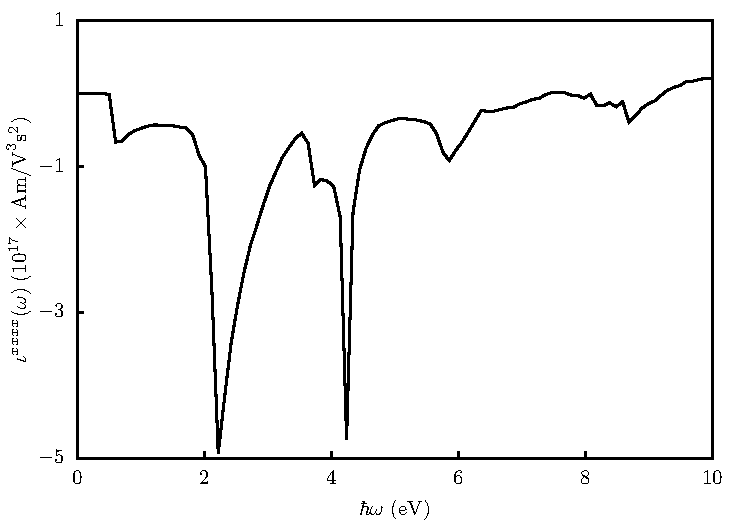
\includegraphics[width=\columnwidth]{jc/jc_GaAs_xxxx.pdf}
\caption{Jerk current tensor component $\iota^{xxxx}$ for GaAs in the $\hbar\omega\in[0, 10]\;\text{eV}$ range.}
\label{fig:GaAs_jc_xxxx}
\end{figure}
\begin{codebox}{}
\begin{verbatim}
bash:/path/of/your/choice/SsTC/doc/examples/example2$ gnuplot
gnuplot> plot 'GaAs-jc_1111.dat' u ($1):(($2)/1E17) w l
\end{verbatim}
\end{codebox}
Other components can also be visualized by the same means.

The user is encouraged to follow the lines of this example and implement his/her own calculators by using the SsTC routines as a basis.
\section{Suggested practices}
It is a good idea to make use of the \href{https://www.intel.com/content/www/us/en/docs/fortran-compiler/developer-guide-reference/2023-0/block.html}{BLOCK} scoping unit in the main application when defining tasks,
\begin{codebox}{}
\begin{lstlisting}[caption={Definition of SsTC tasks in BLOCK scoping units.},captionpos=b]
...
block

  type(optical_BZ_integral_task) :: jerk

  call jerk_current_constructor(optical_task = jerk, method = "rectangle", &
                                samples = (/100, 100, 100/), &
                                omegastart = 0.0_dp, omegaend = 10.0_dp, &
                                omegasteps = 100)

  call SsTC_sample_and_integrate_BZ_integral_task(task = jerk, &
                                                  system = GaAs)

  call SsTC_print_BZ_integral_task(task = jerk, &
                                   system = GaAs)

end block
...
\end{lstlisting}
\end{codebox}
these allow for efficient memory usage, especially if multiple tasks are going to be run. It also helps with derived type finalization. If any component of \verb|task| is going to be used further in the application, creating a copy of the component to a global variable within the application scoping unit is suggested.
\bibliographystyle{unsrt}
\bibliography{bibdata}
\end{document}
